\documentclass[10pt]{beamer}

% Packages
\usepackage[utf8]{inputenc}
\usepackage[T1]{fontenc}
\usepackage{amsmath, amssymb, amsthm}
\usepackage{graphicx}
\usepackage{booktabs}
\usepackage{hyperref}
\usepackage{tikz}
\usetikzlibrary{trees, positioning, shapes, arrows.meta, patterns, decorations.pathreplacing}

\usepackage{algorithm}
\usepackage{algpseudocode}

% Theme settings
\usetheme{default}
\usecolortheme{default}
\usefonttheme{professionalfonts}

% Color definitions (minimalist academic palette)
\definecolor{ThemeBlue}{RGB}{0, 62, 116}
\definecolor{DarkGray}{RGB}{51, 51, 51}
\definecolor{LightGray}{RGB}{245, 245, 245}
\definecolor{AccentOrange}{RGB}{214, 96, 77}
\definecolor{LightBlue}{RGB}{200, 220, 240}
\definecolor{LightOrange}{RGB}{255, 220, 200}
\definecolor{LightGreen}{RGB}{200, 240, 200}
\definecolor{AccentGreen}{RGB}{46, 139, 87}
\definecolor{AccentRed}{RGB}{178, 34, 34}

% Apply colors
\setbeamercolor{frametitle}{fg=ThemeBlue, bg=white}
\setbeamercolor{title}{fg=ThemeBlue}
\setbeamercolor{structure}{fg=ThemeBlue}
\setbeamercolor{normal text}{fg=DarkGray}
\setbeamercolor{block title}{fg=white, bg=ThemeBlue}
\setbeamercolor{block body}{fg=DarkGray, bg=LightGray}
\setbeamercolor{itemize item}{fg=ThemeBlue}
\setbeamercolor{enumerate item}{fg=ThemeBlue}

% Remove navigation symbols
\setbeamertemplate{navigation symbols}{}

% Customize frame title
\setbeamertemplate{frametitle}{
  \vspace{0.5em}
  \insertframetitle
  \vspace{0.3em}
}

% Customize itemize
\setbeamertemplate{itemize items}[circle]
\setlength{\leftmargini}{1.5em}

% Footer
\setbeamertemplate{footline}{
  \leavevmode%
  \hbox{%
  \begin{beamercolorbox}[wd=.333333\paperwidth,ht=2.25ex,dp=1ex,left]{author in head/foot}%
    \hspace{1em}\usebeamerfont{author in head/foot}\insertshortauthor
  \end{beamercolorbox}%
  \begin{beamercolorbox}[wd=.333333\paperwidth,ht=2.25ex,dp=1ex,center]{title in head/foot}%
    \usebeamerfont{title in head/foot}\insertshorttitle
  \end{beamercolorbox}%
  \begin{beamercolorbox}[wd=.333333\paperwidth,ht=2.25ex,dp=1ex,right]{date in head/foot}%
    \usebeamerfont{date in head/foot}\insertshortdate{}\hspace*{2em}
    \insertframenumber{} / \inserttotalframenumber\hspace*{2ex}
  \end{beamercolorbox}}%
  \vskip0pt%
}

% Title page customization
\setbeamertemplate{title page}{
  \vbox{}
  \vfill
  \begingroup
    \centering
    {\usebeamercolor[fg]{title}\usebeamerfont{title}\inserttitle\par}
    \vskip0.5em
    {\usebeamercolor[fg]{subtitle}\usebeamerfont{subtitle}\insertsubtitle\par}
    \vskip2em
    {\usebeamercolor[fg]{author}\usebeamerfont{author}\insertauthor\par}
    \vskip0.5em
    {\usebeamercolor[fg]{institute}\usebeamerfont{institute}\insertinstitute\par}
    \vskip1em
    {\usebeamercolor[fg]{date}\usebeamerfont{date}\insertdate\par}
  \endgroup
  \vfill
}

% Commands for highlighting
\newcommand{\highlight}[1]{\textcolor{AccentOrange}{\textbf{#1}}}
\newcommand{\highlightgreen}[1]{\textcolor{AccentGreen}{\textbf{#1}}}
\newcommand{\highlightred}[1]{\textcolor{AccentRed}{\textbf{#1}}}
\newcommand{\emphbox}[1]{\colorbox{LightGray}{\textcolor{DarkGray}{#1}}}

% Mathematical operators
\DeclareMathOperator*{\argmin}{arg\,min}
\DeclareMathOperator*{\argmax}{arg\,max}
\DeclareMathOperator{\E}{\mathbb{E}}
\DeclareMathOperator{\Var}{Var}
\DeclareMathOperator{\Cov}{Cov}
\DeclareMathOperator{\Corr}{Corr}
\DeclareMathOperator{\MSE}{MSE}
\DeclareMathOperator{\RSS}{RSS}
\DeclareMathOperator{\sign}{sign}

%----------------------------------------------------------------------------------------
% TITLE PAGE
%----------------------------------------------------------------------------------------

\title{Big Data in Finance}
\subtitle{Week 3: Tree-Based Regression Methods}
\author{Dr Daniele Bianchi}
\date{Spring 2026}

%----------------------------------------------------------------------------------------
% DOCUMENT
%----------------------------------------------------------------------------------------

\begin{document}

\AtBeginSection[]{
  \begin{frame}[plain]
    \vfill
    \begin{center}
      {\Large\color{ThemeBlue}\insertsection}
    \end{center}
    \vfill
  \end{frame}
}


% Title slide
\begin{frame}[plain]
  \titlepage
\end{frame}

% Outline slide
\begin{frame}{Today's Agenda}
  \tableofcontents
\end{frame}

%----------------------------------------------------------------------------------------
\section{From Linear to Non-Linear Models}
%----------------------------------------------------------------------------------------

\begin{frame}{Recap: Linear Regression Methods}
  \textbf{Lecture 2:} Given that $f(X) = X^\top\boldsymbol{\beta}$, how do we estimate $\boldsymbol{\beta}$ well?

  \vspace{1em}
  \begin{itemize}
    \item \textbf{OLS:} Unbiased but high variance in high dimensions (overfitting)
    \vspace{0.5em}
    \item \textbf{Ridge:} Shrinks coefficients toward zero (bias for variance)
    \vspace{0.5em}
    \item \textbf{Lasso:} Shrinks + selects variables (sparse solutions)
    \vspace{0.5em}
    \item \textbf{Elastic Net:} Combines L1 and L2 penalties
  \end{itemize}

  \vspace{1em}
  \begin{block}{Common Assumption!}
    All methods assume the true relationship is \highlight{linear in the set of features}
  \end{block}
\end{frame}

%----------------------------------------------------------------------------------------

\begin{frame}{What If Linearity Fails?}
  \textbf{This Lecture:} What if $f(X) \neq X^\top\boldsymbol{\beta}$? How do we let the \highlight{data reveal} the functional form?

  \vspace{1em}
Limitations of linear models:
  \begin{enumerate}
    \item \textbf{Linearity:} Effect of $X_j$ on $Y$ is constant across all values of $X_j$
    \vspace{0.3em}
    \item \textbf{Additivity:} Effect of $X_j$ does not depend on values of other predictors
    \vspace{0.3em}
    \item \textbf{Global model:} Same coefficients everywhere in feature space
  \end{enumerate}

  \vspace{1em}
We can add polynomials ($X_j^2$) and interactions ($X_j\cdot X_i$) manually, but:
  \begin{itemize}
    \item Which ones? How many?
    \item Model dimension explodes with many predictors
  \end{itemize}
\end{frame}

%----------------------------------------------------------------------------------------

\begin{frame}{Think of Equity Premium Prediction}
  \textbf{Goyal-Welch setting:} Predict excess market return using macro predictors

  \vspace{0.5em}
  \begin{itemize}
    \item \textbf{Non-linear effects:}
    \begin{itemize}
      \item Dividend yield may predict differently at extremes
      \item Valuation ratios: effect may saturate
    \end{itemize}

    \vspace{0.5em}
    \item \textbf{Interactions matter:}
    \begin{itemize}
      \item D/P predicts better when term spread is high?
      \item Inflation interacts with real rates
    \end{itemize}

    \vspace{0.5em}
    \item \textbf{Regime dependence:}
    \begin{itemize}
      \item Predictability varies: recessions vs.\ expansions
      \item Different models for different market states
    \end{itemize}
  \end{itemize}

  \vspace{0.5em}
  \begin{block}{Key Question}
    Can we let the data \highlight{discover} which predictors matter where?
  \end{block}
\end{frame}

%----------------------------------------------------------------------------------------


\begin{frame}{The Tree Alternative}
  \textbf{Core idea:} Partition the feature space into regions, fit simple models within each region

  \vspace{1em}
  \begin{columns}[T]
    \column{0.45\textwidth}
    \textbf{Linear Model:}
    \[
    \widehat{f}(x) = \widehat{\beta}_0 + \sum_{j=1}^{p} \widehat{\beta}_j x_j
    \]
    \begin{itemize}
      \item Global: same $\beta$ everywhere
      \item Smooth predictions
      \item Extrapolates beyond data
    \end{itemize}

    \column{0.45\textwidth}
    \textbf{Tree Model:}
    \[
    \widehat{f}(x) = \sum_{m=1}^{M} \widehat{c}_m \cdot \mathbf{1}(x \in R_m)
    \]
    \begin{itemize}
      \item Local: different prediction by averaging returns in a given region $R_m$
      \item Piecewise constant
      \item Cannot extrapolate
    \end{itemize}
  \end{columns}

  \vspace{1.5em}
\highlight{Important Trade-off:} Flexibility vs.\ smoothness
\end{frame}

%----------------------------------------------------------------------------------------
\section{Regression Trees}
%----------------------------------------------------------------------------------------

\begin{frame}{Decision Trees: The Basic Idea}

  \begin{center}
  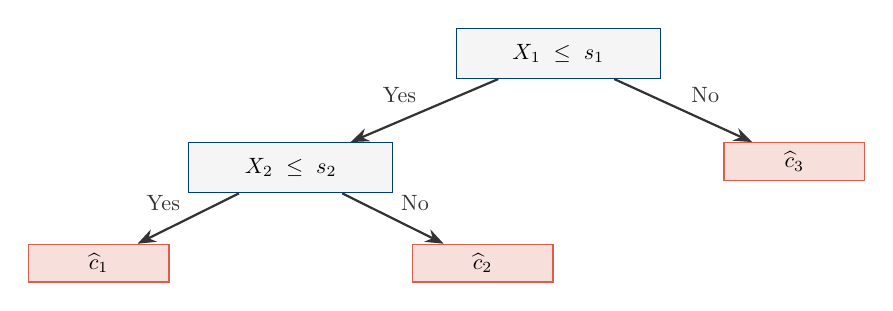
\begin{tikzpicture}[
    scale=0.8, transform shape,
    node distance=1.2cm,
    decision/.style={rectangle, draw=ThemeBlue, fill=LightGray, text width=3cm, text centered, minimum height=0.8cm},
    leaf/.style={rectangle, draw=AccentOrange, fill=AccentOrange!20, text width=2cm, text centered, minimum height=0.6cm},
    arrow/.style={-{Stealth}, thick, DarkGray}
  ]
    \node[decision] (root) {$X_1 \leq s_1$};
    \node[decision, below left=1cm and 1cm of root] (left) {$X_2 \leq s_2$};
    \node[leaf, below right=1cm and 1cm of root] (r1) {$\widehat{c}_3$};
    \node[leaf, below left=0.8cm and 0.3cm of left] (r2) {$\widehat{c}_1$};
    \node[leaf, below right=0.8cm and 0.3cm of left] (r3) {$\widehat{c}_2$};

    \draw[arrow] (root) -- node[above left] {Yes} (left);
    \draw[arrow] (root) -- node[above right] {No} (r1);
    \draw[arrow] (left) -- node[above left] {Yes} (r2);
    \draw[arrow] (left) -- node[above right] {No} (r3);
  \end{tikzpicture}
  \end{center}

  \vspace{0.5em}
  \begin{itemize}
    \item \textbf{Internal nodes:} Binary split on one variable
    \item \textbf{Terminal nodes (leaves):} Predict constant $\widehat{c}_m = \overline{y}_{R_m}$ (mean of training $y$ in region)
  \end{itemize}
\end{frame}

%----------------------------------------------------------------------------------------

\begin{frame}{The Prediction Function}
  A regression tree partitions feature space into $M$ disjoint regions $R_1, \ldots, R_M$

  \vspace{0.5em}
  \textbf{Prediction function:}
  \[
  \widehat{f}(x) = \sum_{m=1}^{M} \widehat{c}_m \cdot \mathbf{1}(x \in R_m)
  \]

  \vspace{0.5em}
  \textbf{Optimal constant within each region:}
  \[
  \widehat{c}_m = \frac{1}{n_m} \sum_{x_i \in R_m} y_i = \overline{y}_{R_m}
  \]

  (minimizes squared error within region)

  \vspace{1em}
  \begin{block}{Key Property}
    Given the partition $\{R_m\}$, the optimal predictions are just \highlight{regional averages}
  \end{block}
\end{frame}

%----------------------------------------------------------------------------------------

\begin{frame}{Finding the Optimal Partition}
  \textbf{Ideal objective:} Find partition minimizing total RSS
  \[
  \min_{\{R_m\}_{m=1}^{M}} \sum_{m=1}^{M} \sum_{x_i \in R_m} (y_i - \widehat{c}_m)^2
  \]

  \vspace{0.5em}
  \textbf{Problem:} Computationally infeasible to search all possible partitions

  \vspace{1em}
  \textbf{Solution:} Greedy recursive binary splitting
  \begin{itemize}
    \item Start with all data in one region
    \item Find the \highlight{single best split} (one variable, one threshold)
    \item Repeat recursively on each resulting region
    \item Stop when criterion met (e.g., minimum leaf size).
  \end{itemize}

  \vspace{0.5em}
  \begin{block}{What Does ``Greedy'' Mean?}
    Pick the best split \textit{right now} without looking ahead---like always taking the immediate shortcut without checking if a longer route would be faster overall
  \end{block}
\end{frame}


%----------------------------------------------------------------------------------------

\begin{frame}{The Splitting Criterion}
  \textbf{At each node}, find split $(j, s)$ minimizing:
  \[
  \min_{j, s} \left[ \sum_{x_i \in R_1(j,s)} (y_i - \widehat{c}_1)^2 + \sum_{x_i \in R_2(j,s)} (y_i - \widehat{c}_2)^2 \right]
  \]

  where:
  \begin{align*}
  R_1(j,s) &= \{X \mid X_j \leq s\} \quad \text{(left child)} \\
  R_2(j,s) &= \{X \mid X_j > s\} \quad \text{(right child)}
  \end{align*}

  \vspace{0.5em}
  \textbf{Algorithm:}
  \begin{enumerate}
    \item For each predictor $j = 1, \ldots, p$:
    \begin{itemize}
      \item For each unique value $s$ of $X_j$ in the data:
      \item Compute RSS reduction from split $(j, s)$
    \end{itemize}
    \item Select $(j^*, s^*)$ with largest RSS reduction
  \end{enumerate}

  \vspace{0.5em}
  \textbf{Complexity:} $O(np)$ per split (efficient!)
\end{frame}

%----------------------------------------------------------------------------------------

\begin{frame}{Visual Example: Equity Premium with Two Predictors}
  \textbf{Setup:} Predict excess return $r_{t+1}$ using D/P (dividend-price) and TMS (term spread)

  \vspace{0.5em}
  \begin{center}
  \begin{tikzpicture}[scale=0.85]
    % Axes
    \draw[->] (0,0) -- (7,0) node[right] {D/P};
    \draw[->] (0,0) -- (0,5) node[above] {TMS};

    % Data points (simplified)
    \foreach \x/\y/\c in {0.5/0.5/red, 1/1.5/red, 1.5/0.8/red, 0.8/2/blue, 1.2/3/blue,
                          2.5/1/red, 3/0.5/blue, 3.5/2/blue, 2.8/3.5/blue,
                          4.5/1/blue, 5/2.5/blue, 5.5/1.5/blue, 4.8/4/blue,
                          5.5/3.5/blue, 6/0.8/blue, 6.2/2.5/blue} {
      \fill[\c!70] (\x,\y) circle (2pt);
    }

    % Legend
    \fill[red!70] (0.5,4.5) circle (2pt);
    \node[right, font=\small] at (0.7,4.5) {$r_{t+1} < 0$};
    \fill[blue!70] (0.5,4) circle (2pt);
    \node[right, font=\small] at (0.7,4) {$r_{t+1} > 0$};

    % Axis labels
    \node[below, font=\small] at (1.5,0) {Low};
    \node[below, font=\small] at (5.5,0) {High};
    \node[left, font=\small] at (0,1) {Low};
    \node[left, font=\small] at (0,4) {High};
  \end{tikzpicture}
  \end{center}

  \vspace{0.3em}
  \textbf{Question:} How should we partition this space to predict returns?
\end{frame}

%----------------------------------------------------------------------------------------

\begin{frame}{Step 1: First Split}
  \textbf{Algorithm searches all variables and thresholds:}
  \begin{itemize}
      \item Best split: $\text{D/P} \leq 2.0$
  \end{itemize}

  \begin{columns}[T]
    \column{0.52\textwidth}
    \begin{center}
    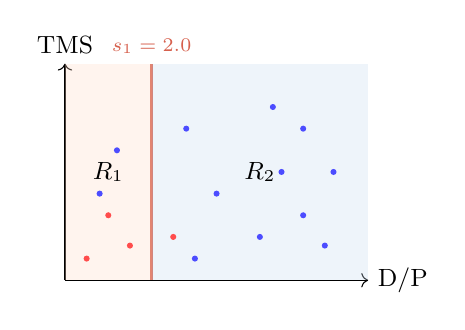
\begin{tikzpicture}[scale=0.55]
      % Axes
      \draw[->] (0,0) -- (7,0) node[right] {\small D/P};
      \draw[->] (0,0) -- (0,5) node[above] {\small TMS};

      % Split line
      \draw[very thick, AccentOrange] (2,0) -- (2,5);
      \node[above, AccentOrange, font=\scriptsize] at (2,5) {$s_1 = 2.0$};

      % Regions
      \fill[LightOrange, opacity=0.3] (0,0) rectangle (2,5);
      \fill[LightBlue, opacity=0.3] (2,0) rectangle (7,5);

      % Region labels
      \node[font=\small] at (1,2.5) {$R_1$};
      \node[font=\small] at (4.5,2.5) {$R_2$};

      % Data points
      \foreach \x/\y/\c in {0.5/0.5/red, 1/1.5/red, 1.5/0.8/red, 0.8/2/blue, 1.2/3/blue,
                            2.5/1/red, 3/0.5/blue, 3.5/2/blue, 2.8/3.5/blue,
                            4.5/1/blue, 5/2.5/blue, 5.5/1.5/blue, 4.8/4/blue,
                            5.5/3.5/blue, 6/0.8/blue, 6.2/2.5/blue} {
        \fill[\c!70] (\x,\y) circle (2pt);
      }
    \end{tikzpicture}
    \end{center}

    \column{0.52\textwidth}
    \begin{center}
    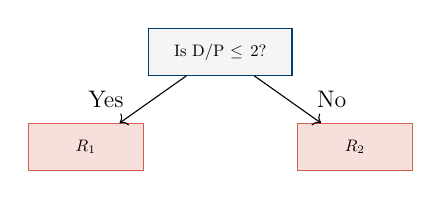
\begin{tikzpicture}[scale=0.6, transform shape,
      decision/.style={rectangle, draw=ThemeBlue, fill=LightGray, text width=2.8cm, text centered, minimum height=1cm},
      leaf/.style={rectangle, draw=AccentOrange, fill=AccentOrange!20, text width=2.2cm, text centered,
      minimum height=1cm}
    ]
      \node[decision] (root) {Is D/P $\leq 2$?};
      \node[leaf, below left=1cm and 0.1cm of root] (l) {$R_1$};
      \node[leaf, below right=1cm and 0.1cm of root] (r) {$R_2$};

      \draw[->] (root) -- node[left=0.5, font=\scriptsize] {\Large Yes} (l);
      \draw[->] (root) -- node[right=0.5, font=\scriptsize] {\Large No} (r);
    \end{tikzpicture}
    \end{center}

    \vspace{0.3em}
    {\footnotesize
    $R_1$: Low D/P\\
    (mostly negative returns)

    \vspace{0.2em}
    $R_2$: High D/P\\
    (mostly positive returns)
    }
  \end{columns}
\end{frame}

%----------------------------------------------------------------------------------------

\begin{frame}{Step 2: Split Left Region}
  \textbf{Now split $R_1$ (low D/P region):}
  \begin{itemize}
    \item Best split: $\text{TMS} \leq 1.5$
  \end{itemize}

  \vspace{0.3em}
  \begin{columns}[T]
    \column{0.55\textwidth}
    \begin{center}
    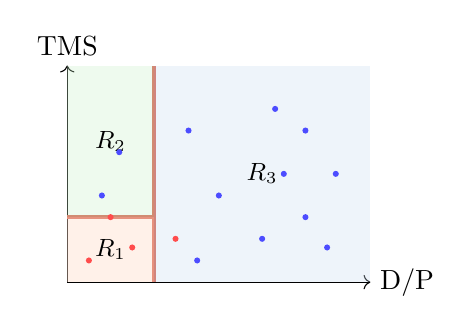
\begin{tikzpicture}[scale=0.55]
      % Axes
      \draw[->] (0,0) -- (7,0) node[right] {D/P};
      \draw[->] (0,0) -- (0,5) node[above] {TMS};

      % Split lines
      \draw[very thick, AccentOrange] (2,0) -- (2,5);
      \draw[very thick, AccentOrange] (0,1.5) -- (2,1.5);

      % Regions
      \fill[LightOrange, opacity=0.4] (0,0) rectangle (2,1.5);
      \fill[LightGreen, opacity=0.3] (0,1.5) rectangle (2,5);
      \fill[LightBlue, opacity=0.3] (2,0) rectangle (7,5);

      % Region labels
      \node[font=\small] at (1,0.75) {$R_1$};
      \node[font=\small] at (1,3.25) {$R_2$};
      \node[font=\small] at (4.5,2.5) {$R_3$};

      % Data points
      \foreach \x/\y/\c in {0.5/0.5/red, 1/1.5/red, 1.5/0.8/red, 0.8/2/blue, 1.2/3/blue,
                            2.5/1/red, 3/0.5/blue, 3.5/2/blue, 2.8/3.5/blue,
                            4.5/1/blue, 5/2.5/blue, 5.5/1.5/blue, 4.8/4/blue,
                            5.5/3.5/blue, 6/0.8/blue, 6.2/2.5/blue} {
        \fill[\c!70] (\x,\y) circle (2pt);
      }
    \end{tikzpicture}
    \end{center}

    \column{0.6\textwidth}
    \begin{center}
    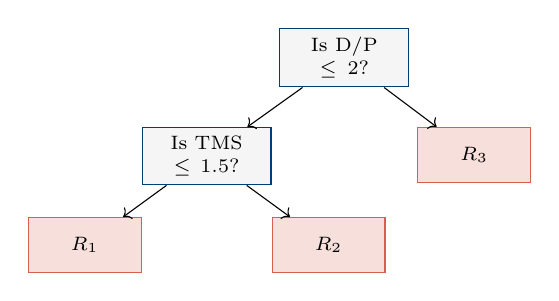
\begin{tikzpicture}[scale=0.4,
      decision/.style={rectangle, draw=ThemeBlue, fill=LightGray, text width=1.4cm, text centered, font=\scriptsize, minimum height=.7cm},
      leaf/.style={rectangle, draw=AccentOrange, fill=AccentOrange!20, text width=1.2cm, text centered, font=\scriptsize,minimum height=.7cm}
    ]
      \node[decision] (root) {Is D/P $\leq 2$?};
      \node[decision, below left=0.5cm and 0.1cm of root] (left) {Is TMS $\leq 1.5$?};
      \node[leaf, below right=0.5cm and 0.1cm of root] (r3) {$R_3$};
      \node[leaf, below left=0.4cm and 0cm of left] (r1) {$R_1$};
      \node[leaf, below right=0.4cm and 0cm of left] (r2) {$R_2$};

      \draw[->] (root) -- (left);
      \draw[->] (root) -- (r3);
      \draw[->] (left) -- (r1);
      \draw[->] (left) -- (r2);
    \end{tikzpicture}
    \end{center}

    \vspace{0.3em}
    {\small
    $R_1$: Low D/P, Low TMS (predict: $-2\%$)

    $R_2$: Low D/P, High TMS (predict: $+1\%$)

    $R_3$: High D/P (predict: $+3\%$)
    }
  \end{columns}
\end{frame}

%----------------------------------------------------------------------------------------

\begin{frame}{Tree Partitions are Axis-Aligned Rectangles}

  \begin{center}
  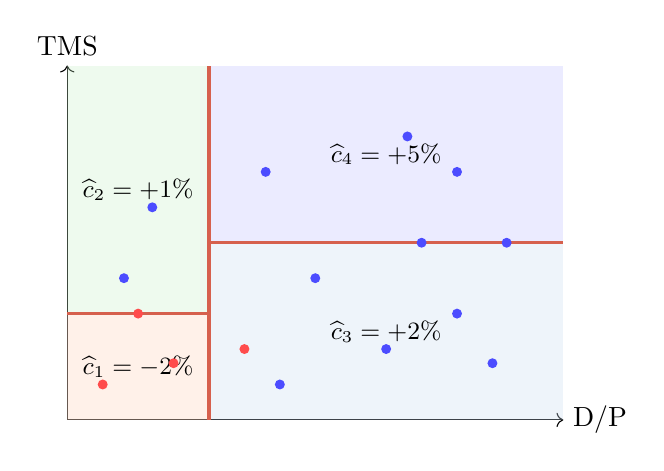
\begin{tikzpicture}[scale=0.9]
    % Axes
    \draw[->] (0,0) -- (7,0) node[right] {D/P};
    \draw[->] (0,0) -- (0,5) node[above] {TMS};

    % Final regions with all splits
    \fill[LightOrange, opacity=0.4] (0,0) rectangle (2,1.5);
    \fill[LightGreen, opacity=0.3] (0,1.5) rectangle (2,5);
    \fill[LightBlue, opacity=0.3] (2,0) rectangle (7,2.5);
    \fill[blue!20, opacity=0.4] (2,2.5) rectangle (7,5);

    % Split lines
    \draw[very thick, AccentOrange] (2,0) -- (2,5);
    \draw[very thick, AccentOrange] (0,1.5) -- (2,1.5);
    \draw[very thick, AccentOrange] (2,2.5) -- (7,2.5);

    % Region labels with predictions
    \node[font=\small] at (1,0.75) {$\widehat{c}_1 = -2\%$};
    \node[font=\small] at (1,3.25) {$\widehat{c}_2 = +1\%$};
    \node[font=\small] at (4.5,1.25) {$\widehat{c}_3 = +2\%$};
    \node[font=\small] at (4.5,3.75) {$\widehat{c}_4 = +5\%$};

    % Data points
    \foreach \x/\y/\c in {0.5/0.5/red, 1/1.5/red, 1.5/0.8/red, 0.8/2/blue, 1.2/3/blue,
                          2.5/1/red, 3/0.5/blue, 3.5/2/blue, 2.8/3.5/blue,
                          4.5/1/blue, 5/2.5/blue, 5.5/1.5/blue, 4.8/4/blue,
                          5.5/3.5/blue, 6/0.8/blue, 6.2/2.5/blue} {
      \fill[\c!70] (\x,\y) circle (2pt);
    }
  \end{tikzpicture}
  \end{center}

  \vspace{0.3em}
  \textbf{Key properties:}
  \begin{itemize}
    \item Splits are always perpendicular to axes (one variable at a time)
    \item Regions are rectangular (in any dimension)
    \item Prediction is \highlight{constant within each region}
  \end{itemize}
\end{frame}

%----------------------------------------------------------------------------------------

\begin{frame}{Interpretation: What the Tree Learned}

  \begin{columns}[T]
    \column{0.5\textwidth}
    \textbf{The fitted tree says:}

    \vspace{0.5em}
    \begin{enumerate}
      \item High D/P $\rightarrow$ positive returns
      \item Low D/P alone $\rightarrow$ depends on TMS
      \item Low D/P + Low TMS $\rightarrow$ negative returns
      \item Low D/P + High TMS $\rightarrow$ mildly positive
    \end{enumerate}

    \vspace{0.5em}
    \textbf{Interaction discovered:}

    TMS matters \textit{only when} D/P is low

    \column{0.5\textwidth}
    \textbf{Compare to linear model:}
    \[
    \widehat{r}_{t+1} = \widehat{\beta}_0 + \widehat{\beta}_1 \text{D/P} + \widehat{\beta}_2 \text{TMS}
    \]

    \begin{itemize}
      \item Effects are additive
      \item Same $\beta_2$ everywhere
      \item Would need to specify $\text{D/P} \times \text{TMS}$ interaction manually
    \end{itemize}
  \end{columns}

  \vspace{0.5em}
  \begin{block}{Trees Automatically Discover}
    \begin{itemize}
      \item Non-linear effects (different predictions at different D/P levels)
      \item Interactions (TMS effect depends on D/P)
    \end{itemize}
  \end{block}
\end{frame}

%----------------------------------------------------------------------------------------

\begin{frame}{When to Stop Splitting?}
  \textbf{Stopping rules} (hyperparameters):

  \vspace{0.5em}
  \begin{itemize}
    \item \textbf{Minimum samples per leaf} (\texttt{min\_samples\_leaf})
    \begin{itemize}
      \item Stop if split would create node with fewer than $k$ observations
      \item Typical: 1--20 for regression
    \end{itemize}

    \vspace{0.5em}
    \item \textbf{Maximum depth} (\texttt{max\_depth})
    \begin{itemize}
      \item Limit number of sequential splits
      \item Typical: 3--20
    \end{itemize}

    \vspace{0.5em}
    \item \textbf{Minimum impurity decrease} (\texttt{min\_impurity\_decrease})
    \begin{itemize}
      \item Stop if RSS reduction below threshold
    \end{itemize}
  \end{itemize}

  \vspace{1em}
  \textbf{Problem:} Early stopping can miss good splits that only become valuable after further splitting
\end{frame}

%----------------------------------------------------------------------------------------

\begin{frame}{Cost-Complexity Pruning}
  \textbf{Better approach:} Grow large tree, then prune back

  \vspace{0.5em}
  \textbf{Cost-complexity criterion:}
  \[
  C_\alpha(T) = \sum_{m=1}^{|T|} \sum_{x_i \in R_m} (y_i - \widehat{c}_m)^2 + \alpha |T|
  \]

  \begin{itemize}
    \item $|T|$ = number of terminal nodes (tree complexity)
    \item $\alpha \geq 0$ = complexity penalty (tuning parameter)
  \end{itemize}

  \vspace{0.5em}
  \begin{block}{Compare to Lasso}
    \begin{tabular}{ll}
      Lasso: & $\RSS + \lambda \sum_j |\beta_j|$ \\
      Tree:  & $\RSS + \alpha |T|$
    \end{tabular}

    \vspace{0.3em}
    Both trade off fit vs.\ complexity; $\alpha$ selected via cross-validation
  \end{block}
\end{frame}

%----------------------------------------------------------------------------------------

\begin{frame}{Bias-Variance Trade-off for Trees}

  \begin{columns}[T]
    \column{0.48\textwidth}
    \textbf{Deep trees:}
    \begin{itemize}
      \item Many small regions
      \item Low bias (can fit complex patterns)
      \item \highlight{High variance} (sensitive to training data)
      \item Risk: overfitting
    \end{itemize}

    \column{0.48\textwidth}
    \textbf{Shallow trees:}
    \begin{itemize}
      \item Few large regions
      \item \highlight{High bias} (may miss patterns)
      \item Low variance (stable)
      \item Risk: underfitting
    \end{itemize}
  \end{columns}

  \vspace{2em}
  \textbf{Key problem:} Single trees are \highlight{notoriously unstable}
  \begin{itemize}
    \item Small change in data $\rightarrow$ completely different tree structure
    \item Different split at root cascades to entire tree
  \end{itemize}

  \vspace{0.5em}
  \centering
  \textit{Can we reduce variance while keeping flexibility?}
\end{frame}

\begin{frame}{Visualizing the Instability Problem}

  \textbf{Illustration:} Same data, two different root splits

  \vspace{0.5em}
 \begin{columns}[T]
    \column{0.48\textwidth}
    \centering
    \textbf{Sample A}
    \vspace{1em}

    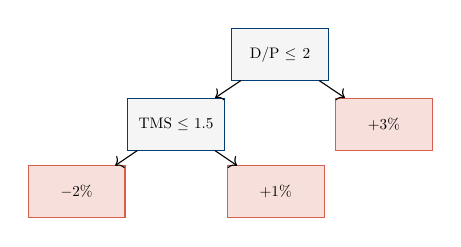
\begin{tikzpicture}[scale=0.55, transform shape,
      decision/.style={rectangle, draw=ThemeBlue, fill=LightGray, text width=2cm, text centered, minimum height=1.2cm},
      leaf/.style={rectangle, draw=AccentOrange, fill=AccentOrange!20, text width=2cm, text centered,
      minimum height=1.2cm}
    ]
      \node[decision] (root) {D/P $\leq 2$};
      \node[decision, below left=0.4cm and 0.15cm of root] (left) {TMS $\leq 1.5$};
      \node[leaf, below right=0.4cm and 0.15cm of root] (r1) {$+3\%$};
      \node[leaf, below left=0.35cm and 0.05cm of left] (r2) {$-2\%$};
      \node[leaf, below right=0.35cm and 0.05cm of left] (r3) {$+1\%$};

      \draw[->] (root) -- (left);
      \draw[->] (root) -- (r1);
      \draw[->] (left) -- (r2);
      \draw[->] (left) -- (r3);
    \end{tikzpicture}

    \column{0.48\textwidth}
    \centering
    \textbf{Sample B}
        \vspace{1em}

    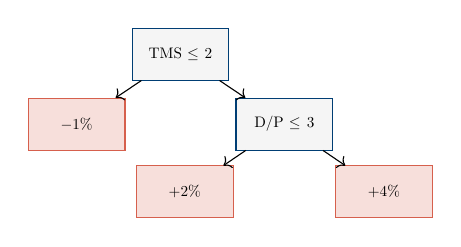
\begin{tikzpicture}[scale=0.55, transform shape,
      decision/.style={rectangle, draw=ThemeBlue, fill=LightGray, text width=2cm, text centered, minimum height=1.2cm},
      leaf/.style={rectangle, draw=AccentOrange, fill=AccentOrange!20, text width=2cm, text centered,
      minimum height=1.2cm}
    ]
      \node[decision] (root) {TMS $\leq 2$};
      \node[leaf, below left=0.4cm and 0.15cm of root] (r1) {$-1\%$};
      \node[decision, below right=0.4cm and 0.15cm of root] (right) {D/P $\leq 3$};
      \node[leaf, below left=0.35cm and 0.05cm of right] (r2) {$+2\%$};
      \node[leaf, below right=0.35cm and 0.05cm of right] (r3) {$+4\%$};

      \draw[->] (root) -- (r1);
      \draw[->] (root) -- (right);
      \draw[->] (right) -- (r2);
      \draw[->] (right) -- (r3);
    \end{tikzpicture}
  \end{columns}

  \vspace{1em}
  \begin{itemize}
    \item High variance in predictions
    \begin{itemize}
        \item Predictions are very sensitive to root splits
    \end{itemize}
    \item This is the cost of flexibility
  \end{itemize}
\end{frame}


%----------------------------------------------------------------------------------------
\section{Ensemble Learning: Bagging, Random Forests, and Boosting}
%----------------------------------------------------------------------------------------

\begin{frame}{The Underlying Intuition}

\textbf{Think about macroeconomic forecasting:}
\begin{itemize}
\item One agency forecast: 60\% accuracy
\item Average forecast from 10 independent agencies: 75\% accuracy
\item Why? Individual forecasting errors tend to cancel out
\end{itemize}
\vspace{2em}

\textbf{The Statistical Principle:}

Given $B$ independent observations $z_1, \ldots, z_B$, each with variance $\sigma^2$:
\begin{align}
\text{Var}(\bar{z}) = \text{Var}\left(\frac{1}{B}\sum_{b=1}^B z_b\right) = \frac{\sigma^2}{B}\notag
\end{align}

Averaging reduces variance by a factor of $B$!


\end{frame}


\begin{frame}{The Challenge: We Don't Have Multiple Datasets}

\textbf{The Problem:}
\begin{itemize}
\item Ideally, we'd train trees on $B$ different training datasets
\item Then average their predictions: $\widehat{f}_{\text{bag}}(x) = \frac{1}{B}\sum_{b=1}^B \widehat{f}^b(x)$
\item But we only have one dataset!
\end{itemize}
\vspace{2em}

\textbf{The Solution: Bootstrap Sampling}
\begin{itemize}
\item Take repeated samples \highlight{with replacement} from our training dataset
\item Each bootstrap sample has the same size as the original data
\item This creates the variation we need for ensemble diversity
\end{itemize}

\end{frame}

\begin{frame}{What Does Bootstrap Sampling Do?}
  \textbf{Bootstrap:} Sample $n$ rows (time periods) \textit{with replacement} from original data

  \vspace{0.3em}
  \begin{center}
  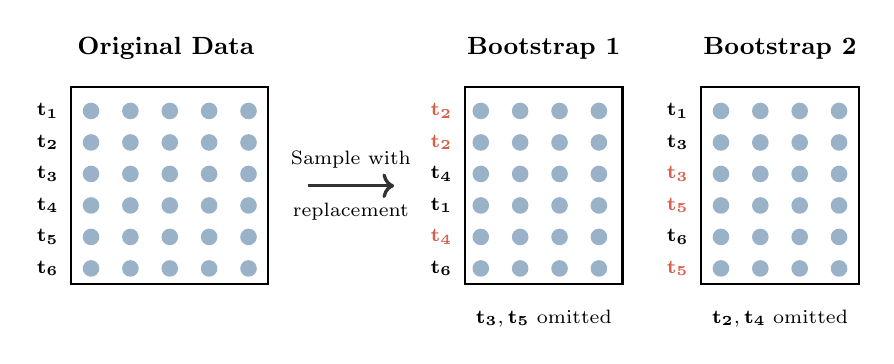
\begin{tikzpicture}[scale=1, transform shape]
    % Original data
    \node[font=\small\bfseries] at (-0.8, 3.5) {Original Data};
    \draw[thick] (-2, 0.5) rectangle (0.5, 3);

    \node[font=\scriptsize] at (-2.3, 2.7) {$\mathbf{t_1}$};
    \node[font=\scriptsize] at (-2.3, 2.3) {$\mathbf{t_2}$};
    \node[font=\scriptsize] at (-2.3, 1.9) {$\mathbf{t_3}$};
    \node[font=\scriptsize] at (-2.3, 1.5) {$\mathbf{t_4}$};
    \node[font=\scriptsize] at (-2.3, 1.1) {$\mathbf{t_5}$};
    \node[font=\scriptsize] at (-2.3, 0.7) {$\mathbf{t_6}$};

    \foreach \y in {2.7, 2.3, 1.9, 1.5, 1.1, 0.7} {
      \fill[ThemeBlue!40] (-1.75, \y) circle (3pt);
      \fill[ThemeBlue!40] (-1.25, \y) circle (3pt);
      \fill[ThemeBlue!40] (-0.75, \y) circle (3pt);
      \fill[ThemeBlue!40] (-0.25, \y) circle (3pt);
      \fill[ThemeBlue!40] (0.25, \y) circle (3pt);
    }

    % Arrow
    \draw[->, very thick, DarkGray] (1, 1.75) -- (2.1, 1.75);
    \node[font=\scriptsize, above] at (1.55, 1.85) {Sample with};
    \node[font=\scriptsize, below] at (1.55, 1.65) {replacement};

    % Bootstrap sample 1
    \node[font=\small\bfseries] at (4, 3.5) {Bootstrap 1};
    \draw[thick] (3, 0.5) rectangle (5, 3);

    \node[font=\scriptsize, AccentOrange] at (2.7, 2.7) {$\mathbf{t_2}$};
    \node[font=\scriptsize, AccentOrange] at (2.7, 2.3) {$\mathbf{t_2}$};
    \node[font=\scriptsize] at (2.7, 1.9) {$\mathbf{t_4}$};
    \node[font=\scriptsize] at (2.7, 1.5) {$\mathbf{t_1}$};
    \node[font=\scriptsize, AccentOrange] at (2.7, 1.1) {$\mathbf{t_4}$};
    \node[font=\scriptsize] at (2.7, 0.7) {$\mathbf{t_6}$};

    \foreach \y in {2.7, 2.3, 1.9, 1.5, 1.1, 0.7} {
      \fill[ThemeBlue!40] (3.2, \y) circle (3pt);
      \fill[ThemeBlue!40] (3.7, \y) circle (3pt);
      \fill[ThemeBlue!40] (4.2, \y) circle (3pt);
      \fill[ThemeBlue!40] (4.7, \y) circle (3pt);
    }

    \node[font=\scriptsize, below] at (4, 0.3) {$\mathbf{t_3}, \mathbf{t_5}$ omitted};

    % Bootstrap sample 2
    \node[font=\small\bfseries] at (7, 3.5) {Bootstrap 2};
    \draw[thick] (6, 0.5) rectangle (8, 3);

    \node[font=\scriptsize] at (5.7, 2.7) {$\mathbf{t_1}$};
    \node[font=\scriptsize] at (5.7, 2.3) {$\mathbf{t_3}$};
    \node[font=\scriptsize, AccentOrange] at (5.7, 1.9) {$\mathbf{t_3}$};
    \node[font=\scriptsize, AccentOrange] at (5.7, 1.5) {$\mathbf{t_5}$};
    \node[font=\scriptsize] at (5.7, 1.1) {$\mathbf{t_6}$};
    \node[font=\scriptsize, AccentOrange] at (5.7, 0.7) {$\mathbf{t_5}$};

    \foreach \y in {2.7, 2.3, 1.9, 1.5, 1.1, 0.7} {
      \fill[ThemeBlue!40] (6.25, \y) circle (3pt);
      \fill[ThemeBlue!40] (6.75, \y) circle (3pt);
      \fill[ThemeBlue!40] (7.25, \y) circle (3pt);
      \fill[ThemeBlue!40] (7.75, \y) circle (3pt);
    }

    \node[font=\scriptsize, below] at (7, 0.3) {$\mathbf{t_2}, \mathbf{t_4}$ omitted};
  \end{tikzpicture}
  \end{center}

  \vspace{0.2em}
  \begin{columns}[T]
    \column{0.55\textwidth}
    \textbf{What happens:}
    \begin{itemize}
      \item Some periods appear multiple times
      \item Some periods are omitted entirely
      \item All $p$ predictors remain
    \end{itemize}

    \column{0.45\textwidth}
    \textbf{Why it helps:}
    \begin{itemize}
      \item Each tree sees different data
      \item Trees make different errors
      \item Averaging reduces variance
    \end{itemize}
  \end{columns}
\end{frame}

%----------------------------------------------------------------------------------------

\begin{frame}{Why Does Averaging Reduce Variance?}
  \textbf{Setup:} $B$ estimators, each with variance $\sigma^2$ and pairwise correlation $\rho$

  \vspace{0.5em}
  \textbf{Variance of average:}
  \[
  \Var\left(\widehat{f}_{\text{bag}}(x)\right)=\Var\left(\frac{1}{B}\sum_{b=1}^{B} \widehat{f}^b(x)\right) = \rho\sigma^2 + \frac{1-\rho}{B}\sigma^2
  \]
  \vspace{0.5em}
  \textbf{As $B \to \infty$ Variance $\to \rho\sigma^2$}

  \vspace{0.5em}
Implications:
  \begin{itemize}
    \item First term depends on \highlight{correlation between trees}
    \item If $\rho = 0$: variance $\to 0$ (ideal)
    \item If $\rho = 1$: no benefit from averaging
    \item \textbf{Issue:} Bootstrap trees are correlated (same predictors across trees)
  \end{itemize}

  \vspace{0.5em}

  \textbf{The Challenge:} How do we ensure our bagged trees are sufficiently different from each other?

\end{frame}

%----------------------------------------------------------------------------------------

\begin{frame}{Two Sources of Randomness in Random Forests}
  Random Forests combine \highlight{two} randomization strategies:

  \vspace{0.5em}
  \begin{center}
  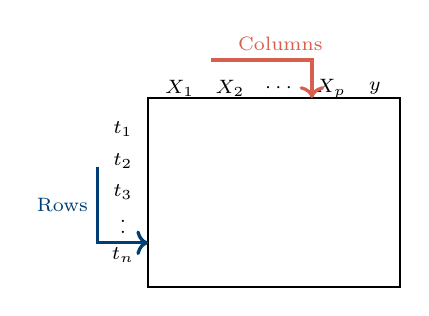
\begin{tikzpicture}[scale=0.8]
    % Data matrix
    \draw[thick] (0,0) rectangle (4,3);
    \node at (2, 3.3) {};

    % Row labels
    \node[font=\scriptsize] at (-0.4, 2.5) {$t_1$};
    \node[font=\scriptsize] at (-0.4, 2.0) {$t_2$};
    \node[font=\scriptsize] at (-0.4, 1.5) {$t_3$};
    \node[font=\scriptsize] at (-0.4, 1.0) {$\vdots$};
    \node[font=\scriptsize] at (-0.4, 0.5) {$t_n$};

    % Column labels
    \node[font=\scriptsize] at (0.5, 3.15) {$X_1$};
    \node[font=\scriptsize] at (1.3, 3.15) {$X_2$};
    \node[font=\scriptsize] at (2.1, 3.15) {$\cdots$};
    \node[font=\scriptsize] at (2.9, 3.15) {$X_p$};
    \node[font=\scriptsize] at (3.6, 3.15) {$y$};

    % Highlight rows
    \draw[very thick, ThemeBlue, ->] (-0.8, 1.9) -- (-0.8, 0.7) -- (0, 0.7);
    \node[font=\scriptsize, ThemeBlue, left] at (-0.8, 1.3) {Rows};

    % Highlight columns
    \draw[very thick, AccentOrange, ->] (1, 3.6) -- (2.6, 3.6) -- (2.6, 3);
    \node[font=\scriptsize, AccentOrange, above] at (2.1, 3.6) {Columns};
  \end{tikzpicture}
  \end{center}

  \vspace{0.3em}
  \begin{columns}[T]
    \column{0.52\textwidth}
    \textbf{\textcolor{ThemeBlue}{1. Bootstrap rows}} (Bagging)
    \begin{itemize}
      \item Sample $n$ time periods with replacement
      \item Some periods repeated, others omitted
      \item $\approx 37\%$ left out (``out-of-bag'')
      \item \textit{Goal:} Create diverse training sets
    \end{itemize}

    \column{0.48\textwidth}
    \textbf{\textcolor{AccentOrange}{2. Subsample columns}} (Random Forest)
    \begin{itemize}
      \item At each split, consider only $m < p$ predictors
      \item Different $m$ predictors each tree
      \item All rows in node still used
      \item \textit{Purpose:} Decorrelate trees
    \end{itemize}
  \end{columns}
\end{frame}

%----------------------------------------------------------------------------------------

\begin{frame}{Visualization: The Random Forest Innovation}
  \textbf{Problem:} Even with bootstrap sampling, trees are correlated

  \vspace{0.3em}
  \begin{center}
  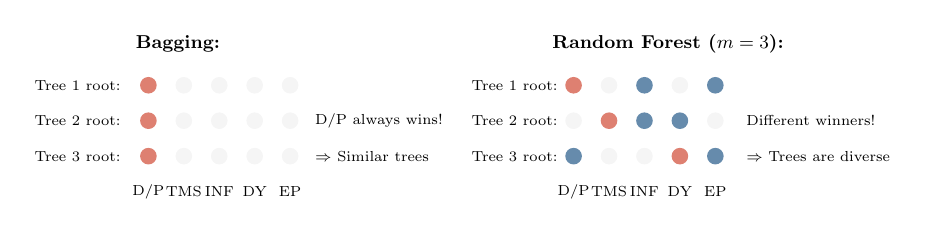
\begin{tikzpicture}[scale=0.75, transform shape]
    % Without subsampling
    \node[font=\small\bfseries] at (-1.5, 2.5) {Bagging:};

    \node[font=\scriptsize] at (-3.2, 1.8) {Tree 1 root:};
    \node[font=\scriptsize] at (-3.2, 1.2) {Tree 2 root:};
    \node[font=\scriptsize] at (-3.2, 0.6) {Tree 3 root:};

    \foreach \y in {1.8, 1.2, 0.6} {
      \fill[AccentOrange!80] (-2, \y) circle (4pt);
      \fill[LightGray] (-1.4, \y) circle (4pt);
      \fill[LightGray] (-0.8, \y) circle (4pt);
      \fill[LightGray] (-0.2, \y) circle (4pt);
      \fill[LightGray] (0.4, \y) circle (4pt);
    }
    \node[font=\scriptsize] at (-2, 0) {D/P};
    \node[font=\scriptsize] at (-1.4, 0) {TMS};
    \node[font=\scriptsize] at (-0.8, 0) {INF};
    \node[font=\scriptsize] at (-0.2, 0) {DY};
    \node[font=\scriptsize] at (0.4, 0) {EP};

    \node[font=\scriptsize, right] at (0.7, 1.2) {D/P always wins!};
    \node[font=\scriptsize, right] at (0.7, 0.6) {$\Rightarrow$ Similar trees};

    % With subsampling
    \node[font=\small\bfseries] at (6.8, 2.5) {Random Forest ($m=3$):};

    \node[font=\scriptsize] at (4.2, 1.8) {Tree 1 root:};
    \node[font=\scriptsize] at (4.2, 1.2) {Tree 2 root:};
    \node[font=\scriptsize] at (4.2, 0.6) {Tree 3 root:};

    % Tree 1: D/P, INF, EP available -> D/P wins
    \fill[AccentOrange!80] (5.2, 1.8) circle (4pt);
    \fill[LightGray] (5.8, 1.8) circle (4pt);
    \fill[ThemeBlue!60] (6.4, 1.8) circle (4pt);
    \fill[LightGray] (7, 1.8) circle (4pt);
    \fill[ThemeBlue!60] (7.6, 1.8) circle (4pt);

    % Tree 2: TMS, INF, DY available -> TMS wins
    \fill[LightGray] (5.2, 1.2) circle (4pt);
    \fill[AccentOrange!80] (5.8, 1.2) circle (4pt);
    \fill[ThemeBlue!60] (6.4, 1.2) circle (4pt);
    \fill[ThemeBlue!60] (7, 1.2) circle (4pt);
    \fill[LightGray] (7.6, 1.2) circle (4pt);

    % Tree 3: D/P, TMS, DY available -> D/P wins
    \fill[ThemeBlue!60] (5.2, 0.6) circle (4pt);
    \fill[LightGray] (5.8, 0.6) circle (4pt);
    \fill[LightGray] (6.4, 0.6) circle (4pt);
    \fill[AccentOrange!80] (7, 0.6) circle (4pt);
    \fill[ThemeBlue!60] (7.6, 0.6) circle (4pt);

    \node[font=\scriptsize] at (5.2, 0) {D/P};
    \node[font=\scriptsize] at (5.8, 0) {TMS};
    \node[font=\scriptsize] at (6.4, 0) {INF};
    \node[font=\scriptsize] at (7, 0) {DY};
    \node[font=\scriptsize] at (7.6, 0) {EP};

    \node[font=\scriptsize, right] at (8, 1.2) {Different winners!};
    \node[font=\scriptsize, right] at (8, 0.6) {$\Rightarrow$ Trees are diverse};
  \end{tikzpicture}
  \end{center}
  {\scriptsize \textcolor{ThemeBlue}{$\bullet$} Available \quad \textcolor{AccentOrange}{$\bullet$} Chosen for split \quad \textcolor{LightGray}{$\bullet$} Not available}

  \vspace{1.3em}
  \textbf{Result:} Lower correlation $\rho$ between trees $\Rightarrow$ lower $\Var\left(\widehat{f}_{\text{bag}}(x)\right)$

  \vspace{0.2em}
  \textbf{Typical:} $m \approx \sqrt{p}$
\end{frame}

%----------------------------------------------------------------------------------------

\begin{frame}{Out-of-Bag (OOB) Error: From Bootstrap Sampling}
  \textbf{Recall:} We bootstrap time periods (rows) with replacement

  \vspace{0.3em}
  \begin{center}
  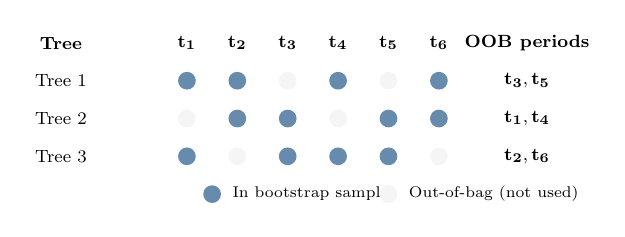
\begin{tikzpicture}[scale=0.8, transform shape]
    % Header
    \node[font=\footnotesize\bfseries] at (-1.2, 2) {Tree};
    \node[font=\footnotesize] at (0.8, 2) {$\mathbf{t_1}$};
    \node[font=\footnotesize] at (1.6, 2) {$\mathbf{t_2}$};
    \node[font=\footnotesize] at (2.4, 2) {$\mathbf{t_3}$};
    \node[font=\footnotesize] at (3.2, 2) {$\mathbf{t_4}$};
    \node[font=\footnotesize] at (4.0, 2) {$\mathbf{t_5}$};
    \node[font=\footnotesize] at (4.8, 2) {$\mathbf{t_6}$};
    \node[font=\footnotesize\bfseries] at (6.2, 2) {OOB periods};

    % Tree 1
    \node[font=\footnotesize] at (-1.2, 1.4) {Tree 1};
    \fill[ThemeBlue!60] (0.8, 1.4) circle (4pt);
    \fill[ThemeBlue!60] (1.6, 1.4) circle (4pt);
    \fill[LightGray] (2.4, 1.4) circle (4pt);
    \fill[ThemeBlue!60] (3.2, 1.4) circle (4pt);
    \fill[LightGray] (4.0, 1.4) circle (4pt);
    \fill[ThemeBlue!60] (4.8, 1.4) circle (4pt);
    \node[font=\footnotesize] at (6.2, 1.4) {$\mathbf{t_3}, \mathbf{t_5}$};

    % Tree 2
    \node[font=\footnotesize] at (-1.2, 0.8) {Tree 2};
    \fill[LightGray] (0.8, 0.8) circle (4pt);
    \fill[ThemeBlue!60] (1.6, 0.8) circle (4pt);
    \fill[ThemeBlue!60] (2.4, 0.8) circle (4pt);
    \fill[LightGray] (3.2, 0.8) circle (4pt);
    \fill[ThemeBlue!60] (4.0, 0.8) circle (4pt);
    \fill[ThemeBlue!60] (4.8, 0.8) circle (4pt);
    \node[font=\footnotesize] at (6.2, 0.8) {$\mathbf{t_1}, \mathbf{t_4}$};

    % Tree 3
    \node[font=\footnotesize] at (-1.2, 0.2) {Tree 3};
    \fill[ThemeBlue!60] (0.8, 0.2) circle (4pt);
    \fill[LightGray] (1.6, 0.2) circle (4pt);
    \fill[ThemeBlue!60] (2.4, 0.2) circle (4pt);
    \fill[ThemeBlue!60] (3.2, 0.2) circle (4pt);
    \fill[ThemeBlue!60] (4.0, 0.2) circle (4pt);
    \fill[LightGray] (4.8, 0.2) circle (4pt);
    \node[font=\footnotesize] at (6.2, 0.2) {$\mathbf{t_2}, \mathbf{t_6}$};

    % Legend
    \fill[ThemeBlue!60] (1.2, -0.4) circle (4pt);
    \node[font=\scriptsize, right] at (1.4, -0.4) {In bootstrap sample};
    \fill[LightGray] (4.0, -0.4) circle (4pt);
    \node[font=\scriptsize, right] at (4.2, -0.4) {Out-of-bag (not used)};
  \end{tikzpicture}
  \end{center}

  \vspace{0.2em}
\textbf{OOB prediction for observation $i$:}
  \[
  \widehat{y}_i^{\text{OOB}} = \frac{1}{|B_i|} \sum_{b \in B_i} T_b(x_i)
  \]
  where $B_i = \{b : \text{observation } i \text{ was OOB for tree } b\}$.

  \vspace{1em}
  \textbf{Example:} Only Tree 2 and 3 see observation $\mathbf{t_3}$ $\Rightarrow$ OOB prediction using Tree 1 (which did not use $\mathbf{t_3}$).

  \vspace{0.3em}
  \begin{block}{Free Cross-Validation!}
    OOB error $\approx$ test error, no need for separate validation set
  \end{block}
\end{frame}

%----------------------------------------------------------------------------------------

\begin{frame}{Summary: The Key Innovation of Random Forest}
  \textbf{Problem:} Bagged trees are correlated (few strong predictors can dominate the splits)

  \vspace{0.3em}
  \textbf{Solution:} \highlight{Decorrelate} the trees (Breiman, 2001)

  \vspace{1em}
  \textbf{Random Forest modification:}

  At each split, consider only a \highlight{random subset} of $m$ predictors

  \vspace{0.5em}
  \begin{itemize}
    \item Before: choose best split among all $p$ predictors
    \item After: choose best split among random $m < p$ predictors
    \item Different random subset at each split
  \end{itemize}

 \vspace{1em}
  \textbf{Recall:} $\Var\left(\widehat{f}_{\text{bag}}(x)\right) = \rho\sigma^2 + \frac{1-\rho}{B}\sigma^2$

  \vspace{0.5em}
  \begin{itemize}
    \item Reducing $\rho$ directly reduces variance
    \item May slightly increase individual tree variance $\sigma^2$ (weaker splits)
    \item Net effect: substantial variance reduction
  \end{itemize}
\end{frame}

%----------------------------------------------------------------------------------------

\begin{frame}{Two Ensemble Strategies}

  \begin{columns}[T]
    \column{0.48\textwidth}
    \textbf{Bagging / Random Forest}
    \begin{itemize}
      \item Build deep trees \highlight{in parallel}
      \item One tree does not depend on another
      \item Combine by averaging
      \item \textbf{Goal:} Variance reduction
    \end{itemize}

    \column{0.48\textwidth}
    \textbf{Boosting}
    \begin{itemize}
      \item Build shallow trees \highlight{sequentially}
      \item Each tree depends on previous
      \item Combine by weighted sum
      \item \textbf{Goal:} Bias reduction
    \end{itemize}
  \end{columns}

  \vspace{1em}
  \begin{block}{Key Insight}
    Bagging: ``Average many overfitting trees to reduce variance''\\
    Boosting: ``Sequentially correct errors of underfitting trees to reduce bias''
  \end{block}
\end{frame}

%----------------------------------------------------------------------------------------

\begin{frame}{Boosting: The Core Idea}
  \textbf{Intuition:} Fit trees to \highlight{residuals} from previous trees

  \vspace{0.5em}
  \begin{enumerate}
    \item Fit a simple tree $\widehat{f}_1(x)$ to data
    \item Compute residuals: $r_i^{(1)} = y_i - \widehat{f}_1(x_i)$
    \item Fit next tree $\widehat{f}_2(x)$ to residuals $r^{(1)}$
    \item Update: $\widehat{f}(x) = \widehat{f}_1(x) + \widehat{f}_2(x)$
    \item Repeat: fit trees to remaining residuals
  \end{enumerate}

  \vspace{0.5em}
  \textbf{Final prediction:}
  \[
  \widehat{f}(x) = \sum_{b=1}^{B} \widehat{f}_b(x)
  \]

  \vspace{0.5em}
  Each tree ``boosts'' the model by correcting mistakes of all previous trees
\end{frame}

%----------------------------------------------------------------------------------------

\begin{frame}{Gradient Boosting: Formal Framework}
  \textbf{View as gradient descent in function space} (Friedman, 2001)

  \vspace{0.3em}
  \textbf{Objective:} Minimize loss $L(y, f(x))$, e.g., squared error
  \[
  \min_f \sum_{i=1}^{n} L(y_i, f(x_i)) = \min_f \sum_{i=1}^{n} (y_i - f(x_i))^2
  \]

  \vspace{0.3em}
  For squared error, the negative gradient is just the \highlight{residual}: $r_i = y_i - f(x_i)$

  \vspace{0.5em}
  \textbf{Concrete example:} Each tree tries to predict the previous residual

  \vspace{0.3em}
  \begin{center}
  \footnotesize
  \begin{tabular}{ccccc}
    \toprule
    \textbf{Iter} & \textbf{Tree target} & \textbf{Tree prediction} & \textbf{Cumulative $\widehat{f}(x_i)$} & \textbf{New residual} \\
    \midrule
    0 & --- & --- & 2\% (mean) & $5\% - 2\% = 3\%$ \\
    1 & 3\% & $h_1(x_i) = 1.5\%$ & $2\% + 1.5\% = 3.5\%$ & $5\% - 3.5\% = 1.5\%$ \\
    2 & 1.5\% & $h_2(x_i) = 0.7\%$ & $3.5\% + 0.7\% = 4.2\%$ & $5\% - 4.2\% = 0.8\%$ \\
    3 & 0.8\% & $h_3(x_i) = 0.4\%$ & $4.2\% + 0.4\% = 4.6\%$ & $5\% - 4.6\% = 0.4\%$ \\
    \bottomrule
  \end{tabular}
  \end{center}

  \vspace{0.3em}
  Each tree corrects remaining errors $\rightarrow$ residuals shrink toward zero
\end{frame}

%----------------------------------------------------------------------------------------

\begin{frame}{The Gradient Boosting Algorithm}

  \begin{algorithm}[H]
  \caption{Gradient Boosting for Regression}
  \begin{algorithmic}[1]
    \State Initialize $\widehat{f}^{(0)}(x) = \bar{y}$ (mean of training targets)
    \For{$b = 1$ to $B$}
      \State Compute residuals: $r_i = y_i - \widehat{f}^{(b-1)}(x_i)$ for all $i$
      \State Fit a shallow tree $h_b(x)$ to residuals $\{(x_i, r_i)\}_{i=1}^n$
      \State Update: $\widehat{f}^{(b)}(x) = \widehat{f}^{(b-1)}(x) + \nu \cdot h_b(x)$
    \EndFor
    \State \textbf{Output:} $\widehat{f}(x) = \widehat{f}^{(B)}(x) = \bar{y} + \nu \sum_{b=1}^{B} h_b(x)$
  \end{algorithmic}
  \end{algorithm}

  \textbf{Key hyperparameters:}
  \begin{itemize}
    \item $B$: number of trees (iterations)
    \item $\nu \in (0,1]$: learning rate (shrinkage) --- typically 0.01--0.1
    \item Tree depth: typically 3--8 (shallow!)
  \end{itemize}

  \begin{block}{Why Shrink? ($\nu < 1$)}
    Small steps prevent overshooting---like turning down the volume on each correction so we do not over-correct and start fitting noise
  \end{block}
\end{frame}

%----------------------------------------------------------------------------------------

\begin{frame}{Why Shallow Trees in Boosting?}

  \textbf{Recall bias-variance:}
  \begin{itemize}
    \item Random Forest: deep trees (low bias) + averaging (reduces variance)
    \item Boosting: shallow trees (high bias) + sequential correction (reduces bias)
  \end{itemize}

  \vspace{0.5em}
  \textbf{Shallow trees (``stumps'' to depth 4--6):}
  \begin{itemize}
    \item High bias individually
    \item But sequential fitting systematically reduces bias
    \item Low variance $\rightarrow$ stable at each step
  \end{itemize}

  \vspace{0.5em}
  \textbf{Tree depth controls interaction order:}
  \begin{itemize}
    \item Depth 1 (stump): only main effects
    \begin{itemize}
      \item Example: ``If D/P $> 2$, predict $+2\%$'' --- no interactions
    \end{itemize}
    \item Depth 2: pairwise interactions
    \begin{itemize}
      \item Example: ``If D/P $> 2$ \textbf{and} TMS $> 1$, predict $+4\%$''
    \end{itemize}
    \item Depth $d$: up to $d$-way interactions
  \end{itemize}

\end{frame}

%----------------------------------------------------------------------------------------

\begin{frame}{Early Stopping: Preventing Overfitting}
  \textbf{Key difference from Random Forest:}
  \begin{itemize}
    \item RF: more trees $\rightarrow$ always helps (or neutral)
    \item Boosting: more trees $\rightarrow$ \highlight{can eventually overfit}
  \end{itemize}

  \vspace{0.3em}
  \textbf{Why?} Each boosting tree is designed to fix remaining errors---eventually it starts fitting noise rather than signal

  \vspace{0.5em}
  \textbf{Solution:} Monitor validation error, stop when it increases

  \vspace{0.3em}
  \begin{center}
  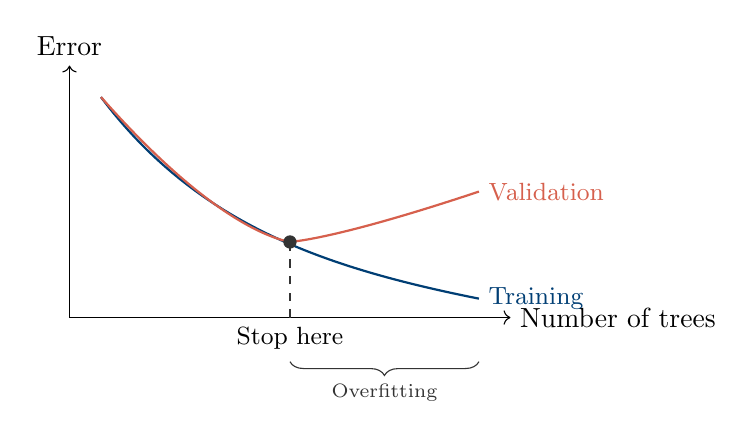
\begin{tikzpicture}[scale=0.8]
    % Axes
    \draw[->] (0,0) -- (7,0) node[right] {Number of trees};
    \draw[->] (0,0) -- (0,4) node[above] {Error};

    % Training error (decreasing)
    \draw[thick, ThemeBlue] (0.5,3.5) .. controls (2,1.5) and (4,0.8) .. (6.5,0.3);
    \node[ThemeBlue, right, font=\small] at (6.5,0.3) {Training};

    % Validation error (U-shaped)
    \draw[thick, AccentOrange] (0.5,3.5) .. controls (2,1.8) and (3,1.3) .. (3.5,1.2)
                               .. controls (4,1.25) and (5,1.5) .. (6.5,2);
    \node[AccentOrange, right, font=\small] at (6.5,2) {Validation};

    % Optimal point
    \draw[dashed, DarkGray] (3.5,0) -- (3.5,1.2);
    \node[below, font=\small] at (3.5,0) {Stop here};
    \fill[DarkGray] (3.5,1.2) circle (3pt);

    % Overfitting region
    \draw[decorate, decoration={brace, amplitude=5pt, mirror}, DarkGray] (3.5,-0.7) -- (6.5,-0.7);
    \node[below, font=\scriptsize, DarkGray] at (5,-0.9) {Overfitting};
  \end{tikzpicture}
  \end{center}

\end{frame}

%----------------------------------------------------------------------------------------

\begin{frame}{RF vs.\ Gradient Boosting: When to Use Which?}

  \begin{center}
  \begin{tabular}{lcc}
    \toprule
    & \textbf{Random Forest} & \textbf{Gradient Boosting} \\
    \midrule
    Tree construction & Parallel (independent) & Sequential (dependent) \\
    Individual trees & Deep (overfit) & Shallow (underfit) \\
    Ensemble goal & Variance reduction & Bias reduction \\
    Overfitting risk & Low & Higher (use early stopping) \\
    Tuning difficulty & Easier & Harder \\
    \bottomrule
  \end{tabular}
  \end{center}

  \vspace{1em}
  \textbf{Practical guidance:}

  \vspace{0.3em}
  \begin{tabular}{ll}
    \textit{Limited tuning time:} & Start with RF (robust to default parameters) \\
    \textit{Maximizing performance:} & Try Boosted trees with careful tuning \\
    \textit{Very noisy data:} & RF (harder to overfit) \\
    \textit{Clear signal, many features:} & Gradient boosting often wins \\
  \end{tabular}

  \vspace{1em}
  \textbf{Hint:} Try both, compare out-of-sample performance
\end{frame}

%----------------------------------------------------------------------------------------
\section{Revisiting Market Timing}
%----------------------------------------------------------------------------------------

\begin{frame}{Recap: What We Learned in Lecture 2}
  \textbf{Market timing with linear methods:}

  \vspace{0.5em}
  \begin{itemize}
    \item OLS overfits badly with many predictors (negative $R^2_{OS}$)
    \item Ridge provided best statistical accuracy ($R^2_{OS}$ closest to zero)
    \item Lasso/Elastic Net behaved like historical mean (always bullish)
    \item Economic performance $\neq$ statistical accuracy
  \end{itemize}

  \vspace{1em}
  \begin{block}{Key Question for Today}
    Can tree-based methods capture \highlight{non-linearities and interactions} that linear models miss?
  \end{block}

  \vspace{0.5em}
  \textbf{Motivation:} Maybe D/P predicts differently at extremes, or the effect of TMS depends on inflation regime
\end{frame}

%----------------------------------------------------------------------------------------

\begin{frame}{The Promise of Tree-Based Methods}
  \textbf{Potential advantages over linear models:}

  \vspace{0.5em}
  \begin{enumerate}
    \item \highlight{Automatic non-linearity:} No need to specify polynomial terms
    \vspace{0.3em}
    \item \highlight{Automatic interactions:} Discovers D/P $\times$ TMS effects without manual coding
    \vspace{0.3em}
    \item \highlight{No scaling required:} Trees are scale-invariant
  \end{enumerate}

  \vspace{1em}
  \textbf{Potential disadvantages:}
  \begin{itemize}
    \item Higher variance (especially single trees)
    \item Hard to extrapolate beyond training data
    \item More hyperparameters to tune
    \item Not particularly effective with noisy data
  \end{itemize}

  \vspace{0.5em}
  \textbf{Empirical question:} Do these advantages outweigh disadvantages for market timing?
\end{frame}

%----------------------------------------------------------------------------------------

\begin{frame}{Implementation: Methods Compared}
  \textbf{Linear methods (from Lecture 2):}
  \begin{itemize}
    \item OLS, Ridge, Lasso, Elastic Net
  \end{itemize}

  \vspace{0.5em}
  \textbf{Tree-based methods (new):}
  \begin{itemize}
    \item \textbf{Decision Tree:} Single pruned tree
    \item \textbf{Random Forest:} Bagging + feature subsampling
    \item \textbf{Gradient Boosting:} Sequential residual fitting
  \end{itemize}

  \vspace{0.5em}
  \textbf{Common setup:}
  \begin{itemize}
    \item Walk-forward prediction (expanding window)
    \item Initial training: 120 months (10 years)
    \item Hyperparameters: Time-series cross-validation
  \end{itemize}

  \vspace{0.5em}
  \textbf{Data:} GWZ (2024) --- 25 predictors, monthly excess returns 1953--2021
\end{frame}

%----------------------------------------------------------------------------------------
\section{Implementing Regression Trees}
%----------------------------------------------------------------------------------------

\begin{frame}{Single Tree Hyperparameters}
  \textbf{Key hyperparameters for regularization:}

  \vspace{0.5em}
  \begin{tabular}{lll}
    \toprule
    \textbf{Parameter} & \textbf{Effect} & \textbf{Grid} \\
    \midrule
    \texttt{max\_depth} & Limits tree depth & \{2, 3, 4, 5, 6\} \\
    \texttt{min\_samples\_leaf} & Min.\ observations per leaf & \{5, 10, 20\} \\
    \bottomrule
  \end{tabular}

  \vspace{1em}
  \textbf{Why constrain depth?}
  \begin{itemize}
    \item The deeper the tree, the more the model overfits
    \item Shallow trees = simpler, more stable rules
    \item Market timing: probably only need 2--3 key fundamental interactions
  \end{itemize}

  \vspace{0.5em}
  \textbf{Selection:} Time-series cross-validation (no shuffling!)
\end{frame}

%----------------------------------------------------------------------------------------

\begin{frame}{Random Forest Hyperparameters}
  \textbf{Key hyperparameters:}

  \vspace{0.3em}
  \begin{tabular}{lll}
    \toprule
    \textbf{Parameter} & \textbf{Effect} & \textbf{Grid} \\
    \midrule
    \texttt{n\_estimators} & Number of trees & 100 (fixed) \\
    \texttt{max\_depth} & Individual tree depth & \{3, 5, 7, None\} \\
    \texttt{max\_features} & Features per split & \{$\sqrt{p}$, 0.33, 0.5\} \\
    \texttt{min\_samples\_leaf} & Min.\ observations per leaf & \{5, 10, 20\} \\
    \bottomrule
  \end{tabular}

  \vspace{0.5em}
  \textbf{Key insight:} More trees never hurts (just slower)

  \vspace{0.3em}
  Focus tuning on:
  \begin{itemize}
    \item \texttt{max\_features}: controls tree correlation (lower $\to$ more diverse)
    \item \texttt{max\_depth}: controls individual tree complexity (deeper tree $\to$ overfitting)
  \end{itemize}
\end{frame}

%----------------------------------------------------------------------------------------

\begin{frame}{Gradient Boosting Hyperparameters}
  \textbf{Key hyperparameters:}

  \vspace{0.3em}
  \begin{tabular}{lll}
    \toprule
    \textbf{Parameter} & \textbf{Effect} & \textbf{Grid} \\
    \midrule
    \texttt{n\_estimators} & Number of boosting rounds & \{50, 100, 200\} \\
    \texttt{max\_depth} & Tree depth (interaction order) & \{2, 3, 4\} \\
    \texttt{learning\_rate} & Shrinkage factor $\nu$ & \{0.01, 0.05, 0.1\} \\
    \bottomrule
  \end{tabular}

  \vspace{0.5em}
  \textbf{Critical trade-off:} \texttt{learning\_rate} $\times$ \texttt{n\_estimators}
  \begin{itemize}
    \item Small $\nu$ + many trees = careful, gradual learning
    \item Large $\nu$ + few trees = aggressive, faster learning
    \item Small $\nu$ generally better but slower
  \end{itemize}

  \vspace{0.3em}
  \textbf{Depth for GBM:} Keep shallow individual trees (2--4) since boosting reduces bias
\end{frame}

%----------------------------------------------------------------------------------------
\section{Out-of-Sample Statistical Performance}
%----------------------------------------------------------------------------------------

\begin{frame}{Out-of-Sample $R^2$: Linear vs.\ Tree Methods}
\textbf{Recall:} $R^2_{OS} = 1 - \frac{\sum_t(r_t - \widehat{r}_t)^2}{\sum_t(r_t - \bar{r}_t)^2}$

  \vspace{0.5em}
  Negative $R^2_{OS}$ means worse than predicting the historical mean.

  \vspace{0.5em}
  \begin{center}
  \begin{tabular}{lcc}
    \toprule
    \textbf{Model} & \textbf{$R^2_{OS}$ (\%)} & \textbf{Assessment} \\
    \midrule
    OLS & $-13.85$ & \highlightred{Severe overfitting} \\
    Ridge & $-0.50$ & Slight underperformance \\
    Lasso & $+0.10$ & $\approx$ Historical mean \\
    Elastic Net & $+0.14$ & $\approx$ Historical mean \\
    \midrule
    Decision Tree & $-10.68$ & \highlightred{Severe overfitting} \\
    \highlightgreen{Random Forest} & $\mathbf{+0.15}$ & \highlightgreen{Best} \\
    Gradient Boosting & $-0.88$ & Moderate overfitting \\
    \bottomrule
  \end{tabular}
  \end{center}

  \vspace{0.3em}
  \textbf{Surprise:} Random Forest achieves the \highlight{only positive} $R^2_{OS}$ among complex models!
\end{frame}

%----------------------------------------------------------------------------------------

\begin{frame}{Interpreting the Results}
  \textbf{Key observations:}

  \vspace{0.5em}
  \begin{enumerate}
    \item \highlight{Single trees overfit dramatically} ($R^2_{OS} = -10.7\%$)
    \begin{itemize}
      \item Worse than OLS in relative terms
      \item Flexibility without ensemble averaging $\to$ noise fitting
    \end{itemize}

    \vspace{0.3em}
    \item \highlight{Random Forest achieves best statistical accuracy}
    \begin{itemize}
      \item Only non-linear model with positive $R^2_{OS}$ (+0.15\%)
      \item Averaging + decorrelation effectively controls variance
    \end{itemize}

    \vspace{0.3em}
    \item \highlight{Gradient Boosting disappoints} ($R^2_{OS} = -0.88\%$)
    \begin{itemize}
      \item Sequential bias reduction less useful when signal is weak
      \item Easier to overfit than Random Forest
    \end{itemize}

    \vspace{0.3em}
    \item \highlight{Lasso and E-Net behave like historical mean}
    \begin{itemize}
      \item Shrink most coefficients to zero $\to$ predict near-constant
    \end{itemize}
  \end{enumerate}
\end{frame}

%----------------------------------------------------------------------------------------

\begin{frame}{Cumulative Squared Error Differential}
  \begin{center}
    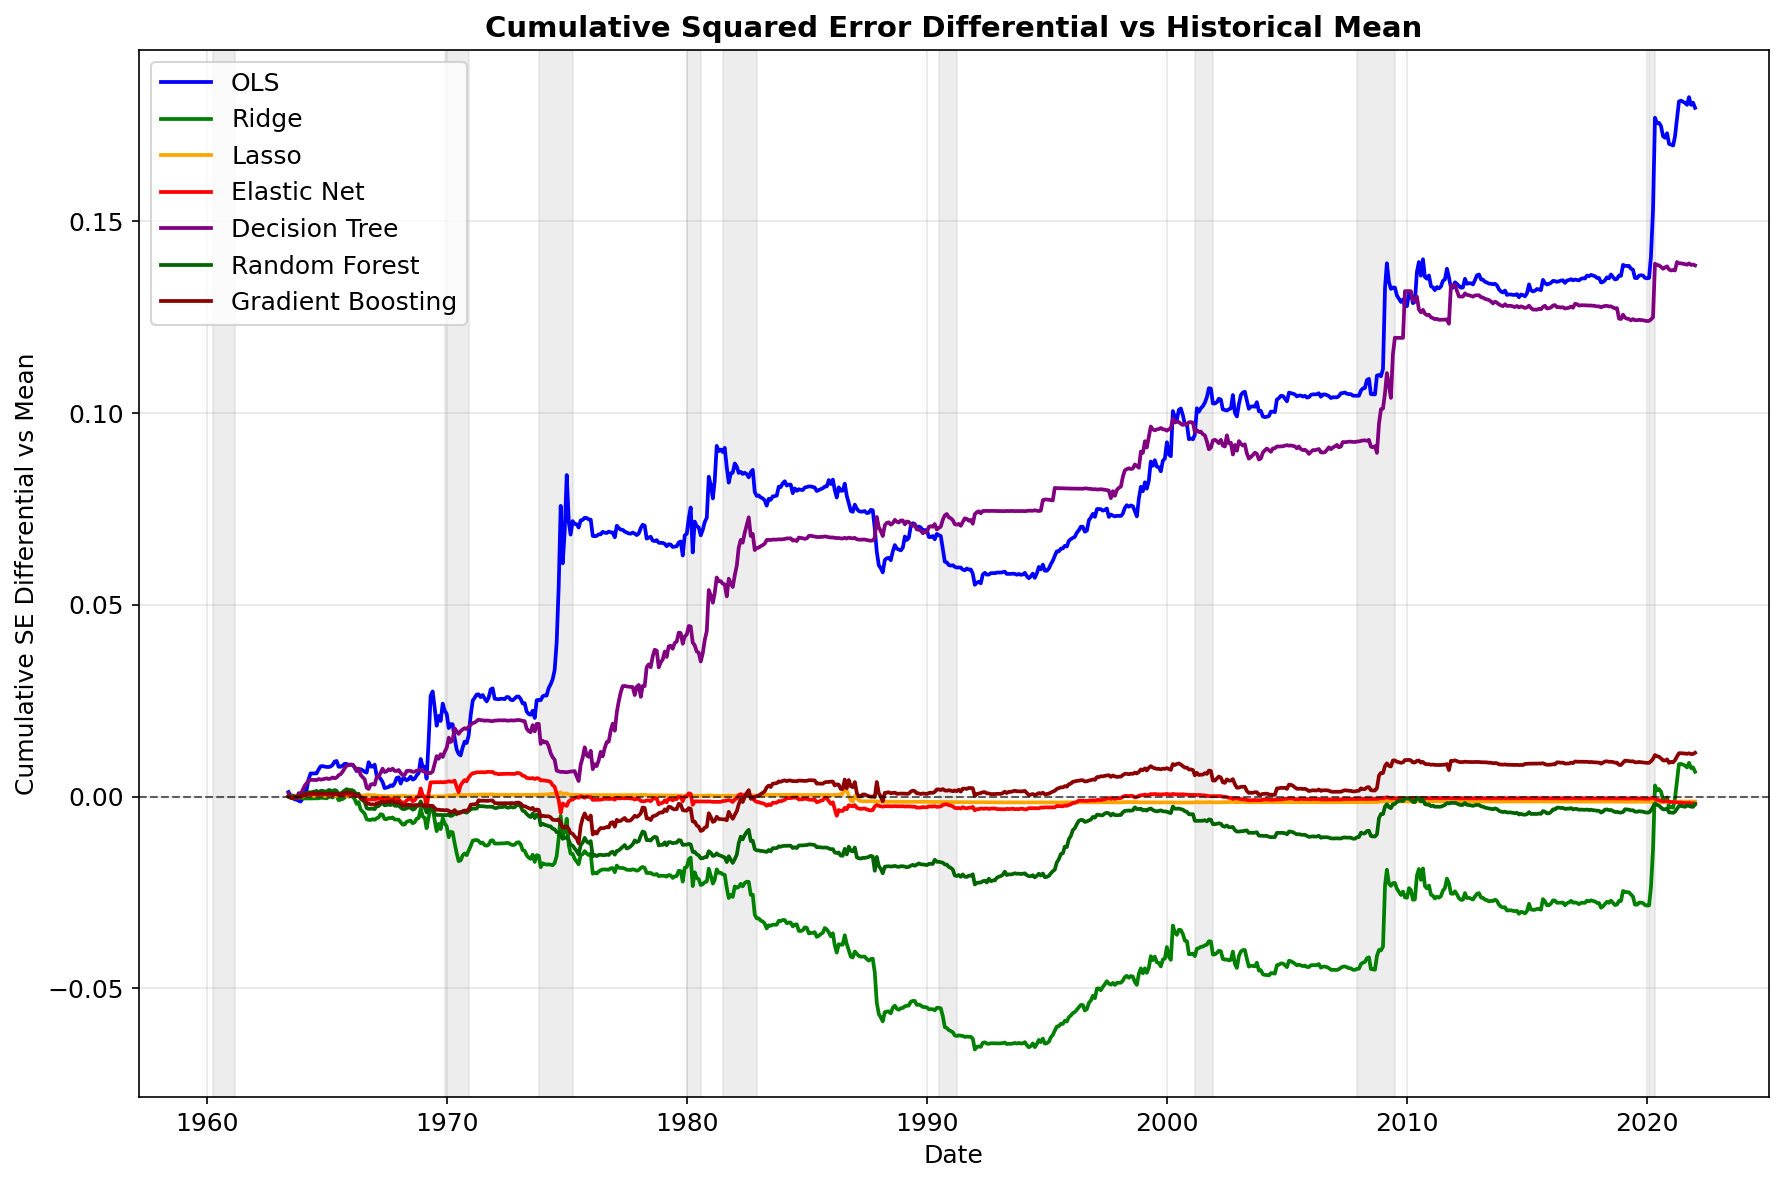
\includegraphics[width=0.8\textwidth]{Figures/tree_cumulative_sse_differential.png}
  \end{center}

  \vspace{-0.8em}
  {\small
The chart shows the \textbf{cumulative Sum of Squared Error (SSE)} difference: $\sum_{t=1}^T [(y_t - \widehat{y}_t^{\text{model}})^2 - (y_t - \bar{y}_t)^2]$

  \begin{itemize}
    \item \highlight{Below zero} = model beats historical mean
    \item \highlight{Above zero} = model worse than historical mean
  \end{itemize}
  }
\end{frame}

%----------------------------------------------------------------------------------------

\begin{frame}{Cumulative SSE Differential: What We Learn}

   \textbf{Key patterns in the figure:}
  \begin{enumerate}
    \item \highlightred{OLS \& Decision Tree}: Steadily accumulate errors, especially during crises
    \item \highlightgreen{Ridge \& Random Forest}: Fluctuate but consistently below zero
    \item \textbf{Lasso/Elastic Net/GBM}: Flat near zero (predictions $\approx$ historical mean)
  \end{enumerate}

  \vspace{0.5em}
  \textbf{Timing insight:} Large jumps occur during volatile periods (gray bands = recessions)
  \begin{itemize}
    \item 2008--2009 crisis: OLS predictions particularly bad
  \end{itemize}
\end{frame}

%----------------------------------------------------------------------------------------

\begin{frame}{Sign Accuracy: Getting the Direction Right}
  \textbf{Sign accuracy:} \% of months where predicted sign = actual sign

\begin{center}
\renewcommand{\arraystretch}{1}
\resizebox{1\textwidth}{!}{\begin{tabular}{lccc}
    \toprule
    \textbf{Model} & \textbf{Sign Acc.\ (\%)} & \textbf{When Up (\%)} & \textbf{When Down (\%)} \\
    \midrule
    Historical Mean & 59.4 & 100.0 & 0.0 \\
    \midrule
    OLS & 58.4 & 68.9 & 43.0 \\
    Ridge & 58.1 & 73.2 & 36.0 \\
    \highlightgreen{Lasso} & \textbf{59.5} & 100.0 & 0.3 \\
    Elastic Net & 57.8 & 92.3 & 7.3 \\
    \midrule
    Decision Tree & 56.5 & 74.2 & 30.8 \\
    Random Forest & 58.0 & 82.8 & 21.7 \\
    Gradient Boosting & 56.3 & 86.1 & 12.6 \\
    \bottomrule
  \end{tabular}}
  \end{center}

  \vspace{0.5em}
  \textbf{Key insight:} Lasso achieves highest sign accuracy but is \highlight{always bullish}---same strategy as historical mean.
\end{frame}

%----------------------------------------------------------------------------------------

\begin{frame}{Why Trees Have More Balanced Predictions}
  \textbf{Sparse linear models (Lasso/Elastic Net):}
  \begin{itemize}
    \item Shrink most/all coefficients toward zero
    \item Predictions collapse to near-constant (historical mean)
    \item ``When Down'' accuracy $\approx 0$--7\% (almost never predict negative)
  \end{itemize}

  \vspace{0.5em}
  \textbf{Tree models:}
  \begin{itemize}
    \item ``When Down'' accuracy 13--31\% (do predict some negative months)
  \end{itemize}

  \vspace{0.5em}
  \textbf{OLS/Ridge (unconstrained):}
  \begin{itemize}
    \item Most balanced: ``When Down'' accuracy 36--43\%
    \item But also most volatile predictions $\to$ more trading
  \end{itemize}

  \vspace{0.5em}
  \begin{block}{Trade-off}
    More balanced predictions $\to$ potentially catch downturns\\
    But also $\to$ higher turnover and more false alarms
  \end{block}
\end{frame}

%----------------------------------------------------------------------------------------
\section{Economic Performance}
%----------------------------------------------------------------------------------------

\begin{frame}{From Predictions to Portfolios}
  \textbf{Market timing strategy:} Same as Lecture 2

  \vspace{0.5em}
  \textbf{Mean-variance optimal weight:}
  \[
  \omega_t = \frac{1}{\gamma}\frac{\widehat{r}_{t+1}}{\widehat{\sigma}^2_t}
  \]

  \begin{itemize}
    \item $\gamma = 5$ (risk aversion)
    \item $\widehat{\sigma}^2_t$ = rolling 60-month variance
    \item Constraints: $-1 \leq \omega_t \leq 1.5$
  \end{itemize}

  \vspace{0.5em}
  \textbf{Portfolio return:}
  \[
  r_{t+1}^{\text{portfolio}} = \omega_t \cdot r_{t+1}^{\text{market}} + (1-\omega_t) \cdot r_f
  \]

  \vspace{0.3em}
  \textbf{Transaction costs:} 50 bps per unit weight change
\end{frame}

%----------------------------------------------------------------------------------------

\begin{frame}{Performance Comparison: Sharpe Ratios}

  \begin{center}
  \renewcommand{\arraystretch}{1}
\resizebox{1\textwidth}{!}{\begin{tabular}{lcccc}
    \toprule
    \textbf{Strategy} & \textbf{Ann.\ Ret.\ (\%)} & \textbf{Vol.\ (\%)} & \textbf{Sharpe} & \textbf{Sharpe Net} \\
    \midrule
    Buy \& Hold & 6.9 & 14.8 & 0.46 & 0.46 \\
    Historical Mean & 4.3 & 11.1 & 0.39 & 0.38 \\
    \midrule
    OLS & 11.2 & 17.5 & 0.64 & 0.45 \\
    \highlightgreen{Ridge} & \textbf{11.9} & 17.1 & \textbf{0.69} & \textbf{0.53} \\
    Lasso & 4.6 & 11.6 & 0.40 & 0.39 \\
    Elastic Net & 5.0 & 11.8 & 0.43 & 0.37 \\
    \midrule
    Decision Tree & 6.3 & 16.0 & 0.39 & 0.29 \\
    Random Forest & 7.0 & 14.4 & 0.49 & 0.35 \\
    Gradient Boosting & 5.1 & 14.4 & 0.36 & 0.22 \\
    \bottomrule
  \end{tabular}}
  \end{center}

  \vspace{0.3em}
  \textbf{Key finding:} Ridge dominates economically despite worse $R^2_{OS}$ than RF!

  \vspace{0.3em}
  \textbf{Puzzle:} How can Ridge have negative $R^2_{OS}$ but best returns?
\end{frame}

%----------------------------------------------------------------------------------------

\begin{frame}{Impact of Transaction Costs}
  \textbf{Turnover comparison:}

  \vspace{0.3em}
  \begin{center}
  \renewcommand{\arraystretch}{1}
\resizebox{1\textwidth}{!}{\begin{tabular}{lccc}
    \toprule
    \textbf{Model} & \textbf{Avg.\ Annual Turnover} & \textbf{Sharpe Gross} & \textbf{Sharpe Net} \\
    \midrule
    Historical Mean & 0.13$\times$ & 0.39 & 0.38 \\
    Lasso & 0.19$\times$ & 0.40 & 0.39 \\
    Elastic Net & 1.40$\times$ & 0.43 & 0.37 \\
    \midrule
    Decision Tree & 3.32$\times$ & 0.39 & 0.29 \\
    Random Forest & 3.85$\times$ & 0.49 & 0.35 \\
    Gradient Boosting & 4.08$\times$ & 0.36 & \highlightred{0.22} \\
    \midrule
    Ridge & 5.67$\times$ & 0.69 & \highlightgreen{0.53} \\
    OLS & 6.79$\times$ & 0.64 & 0.45 \\
    \bottomrule
  \end{tabular}}
  \end{center}

  \vspace{0.5em}
  \textbf{Observations:}
  \begin{itemize}
    \item Tree methods have 3--4$\times$ annual turnover
    \item Ridge has highest turnover but still best net Sharpe!
    \item GBM hurt most by costs (Sharpe drops from 0.36 to 0.22)
  \end{itemize}
\end{frame}

%----------------------------------------------------------------------------------------

\begin{frame}{Cumulative Returns}
  \begin{center}
    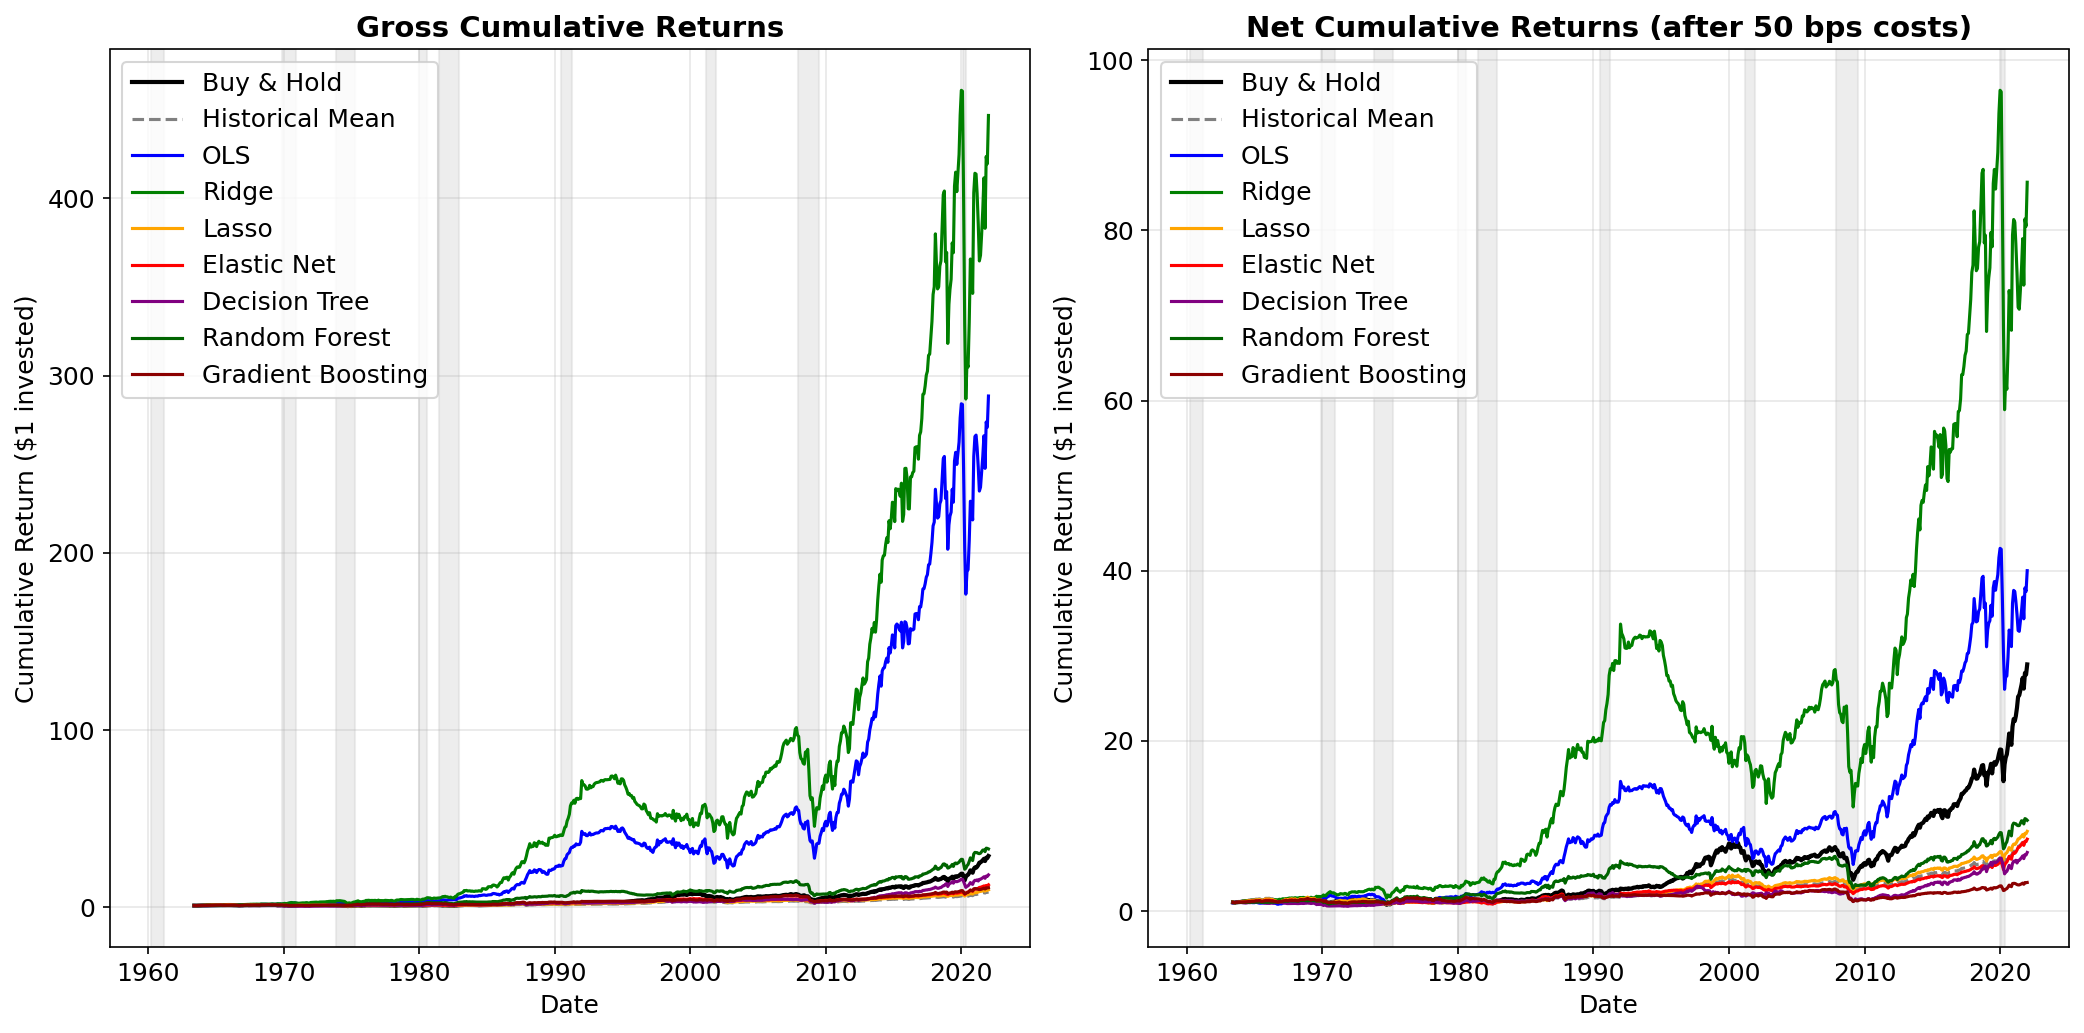
\includegraphics[width=1\textwidth]{Figures/tree_market_timing_cumulative_returns.png}
  \end{center}

  \textbf{Left panel:} Gross returns (no transaction costs)\\ \textbf{Right panel:} Net returns (50 bps costs)
\end{frame}

%----------------------------------------------------------------------------------------

\begin{frame}{Cumulative Returns: What the Figure Shows}

  \textbf{Gross returns (left panel):}
  \begin{itemize}
    \item \highlightgreen{Ridge}: Dominates dramatically, reaches \$400+ by 2021
    \item \textbf{OLS}: Second best gross ($\sim$\$290), but very volatile path
    \item \textbf{Random Forest}: Solid growth ($\sim$\$32), much smoother than OLS
    \item \textbf{All others}: Cluster near bottom (\$5--\$20)
  \end{itemize}

  \vspace{0.5em}
  \textbf{Net returns after 50 bps costs (right panel):}
  \begin{itemize}
    \item \highlightgreen{Ridge}: Still best ($\sim$\$85), but gap narrows substantially
    \item \textbf{Buy \& Hold}: Catches up to $\sim$\$40 (no trading costs)
    \item \textbf{OLS}: Falls to $\sim$\$40 (high turnover penalized)
    \item \textbf{Random Forest}: $\sim$\$10, penalized by 3.85$\times$ turnover
  \end{itemize}

  \vspace{0.5em}
  \begin{block}{Key Insight}
    Ridge's \textit{economic} dominance persists after costs, but the margin shrinks.\\
    Transaction costs matter more for tree methods than linear methods.
  \end{block}
\end{frame}

%----------------------------------------------------------------------------------------

\begin{frame}{The $R^2$ vs.\ Economic Performance Puzzle}
  \textbf{Puzzle:} Random Forest has best $R^2_{OS}$ (+0.15\%), but Ridge has best returns. Why?

  \vspace{0.5em}
  \textbf{Resolution:} $R^2_{OS}$ measures \textit{average} squared error, but economic value depends on:

  \vspace{0.3em}
  \begin{enumerate}
    \item \textbf{Magnitude of correct predictions}
    \begin{itemize}
      \item Ridge makes bigger bets when confident
      \item RF predictions are more muted (closer to zero)
    \end{itemize}

    \vspace{0.2em}
    \item \textbf{Timing of errors}
    \begin{itemize}
      \item Being wrong in calm markets costs less than in volatile markets
      \item Ridge may time the big moves better
    \end{itemize}

    \vspace{0.2em}
    \item \textbf{Portfolio construction}
    \begin{itemize}
      \item Mean-variance weights amplify prediction differences
      \item Small differences in predictions $\to$ big differences in positions
    \end{itemize}
  \end{enumerate}

  \vspace{0.5em}
  \begin{block}{Lesson}
    \highlight{Statistical accuracy $\neq$ Economic value}. Always evaluate both!
  \end{block}
\end{frame}

%----------------------------------------------------------------------------------------

\begin{frame}{Why Don't Trees Dominate?}
  \textbf{We expected trees to help because:}
  \begin{itemize}
    \item They capture non-linearities automatically
    \item They discover interactions without specification
  \end{itemize}

  \vspace{0.5em}
  \textbf{Results show:} RF has best $R^2_{OS}$, but Ridge has best economic performance. Why?

  \vspace{0.5em}
  \begin{enumerate}
    \item \textbf{RF predictions are too conservative}
    \begin{itemize}
      \item Averaging many trees $\to$ predictions shrink toward zero
      \item Good for $R^2$ (small errors), bad for returns (small bets)
    \end{itemize}

    \vspace{0.3em}
    \item \textbf{Ridge takes bigger positions}
    \begin{itemize}
      \item More aggressive forecasts when predictors are extreme
      \item Higher volatility but also higher returns
    \end{itemize}

    \vspace{0.3em}
    \item \textbf{Variance reduction may be too much}
    \begin{itemize}
      \item RF succeeds at variance reduction
      \item But in low signal-to-noise settings, you need some variance to generate returns
    \end{itemize}
  \end{enumerate}
\end{frame}

%----------------------------------------------------------------------------------------

\begin{frame}{The Market Timing Puzzle}
  \textbf{We expected trees to help because:}
  \begin{itemize}
    \item They capture non-linearities automatically
    \item They discover interactions without specification
  \end{itemize}

  \vspace{0.5em}
  \textbf{But results show trees don't clearly outperform Ridge. Why?}

  \vspace{0.5em}
  \begin{enumerate}
    \item \textbf{Signal is too weak}
    \begin{itemize}
      \item Monthly return volatility $\approx 4$--5\%
      \item Predictable component $\approx 0.5\%$ (if any)
      \item Non-linearities in the noise, not the signal
    \end{itemize}

    \vspace{0.3em}
    \item \textbf{Sample size limitations}
    \begin{itemize}
      \item $\sim$800 months may not be enough for complex patterns
      \item Trees need more data than linear models
    \end{itemize}

    \vspace{0.3em}
    \item \textbf{Linear approximation may be sufficient}
    \begin{itemize}
      \item True non-linearities might be small
      \item Occam's razor: simpler models generalize better
    \end{itemize}
  \end{enumerate}
\end{frame}

%----------------------------------------------------------------------------------------

\begin{frame}{When Do Trees Excel?}
  \textbf{Trees tend to outperform when:}

  \vspace{0.5em}
  \begin{enumerate}
    \item \textbf{True interactions exist and are strong}
    \begin{itemize}
      \item Credit risk: income $\times$ debt ratio
      \item Trading: volume $\times$ price momentum
    \end{itemize}

    \vspace{0.3em}
    \item \textbf{Non-linearities are pronounced}
    \begin{itemize}
      \item Threshold effects (default if ratio $> x$)
      \item Saturation effects
    \end{itemize}

    \vspace{0.3em}
    \item \textbf{Sample size is large}
    \begin{itemize}
      \item Cross-sectional prediction: 1000s of stocks per month
      \item More data to detect complex patterns
    \end{itemize}

    \vspace{0.3em}
    \item \textbf{Signal-to-noise ratio is higher}
    \begin{itemize}
      \item Default prediction: $R^2 \approx 10$--30\%
      \item Return prediction: $R^2 \approx 1$--2\%
    \end{itemize}
  \end{enumerate}
\end{frame}

%----------------------------------------------------------------------------------------

\begin{frame}{Gu, Kelly \& Xiu (2020): What the Literature Says}
  \textbf{Cross-sectional return prediction:}
  \begin{itemize}
    \item Trees perform well with firm characteristics
    \item Neural networks slightly better
    \item All ML methods beat linear models
  \end{itemize}

  \vspace{0.5em}
  \textbf{Time-series (market timing):}
  \begin{itemize}
    \item Much harder problem
    \item Trees ``competitive but not dominant''
    \item Gains modest compared to cross-section
  \end{itemize}

  \vspace{0.5em}
  \begin{block}{Key Insight}
    The value of ML depends on the application:
    \begin{itemize}
      \item High signal + large cross-section $\to$ ML helps a lot
      \item Low signal + small time series $\to$ simpler methods suffice
    \end{itemize}
  \end{block}
\end{frame}

%----------------------------------------------------------------------------------------
\section{Summary and Next Steps}
%----------------------------------------------------------------------------------------

\begin{frame}{Key Takeaways from Today}
  \begin{enumerate}
    \item Market timing is very difficult even with non-linear regression models
    \begin{itemize}
      \item Random Forest only modest positive $R^2_{OS}$ (+0.15\%)
      \item Averaging + decorrelation helps to control overfitting
      \item Yet ridge achieves a statistical accuracy ($R^2_{OS}$) just as good as RF
    \end{itemize}
\vspace{0.3em}
     \item Single trees and OLS catastrophically overfit
    \begin{itemize}
      \item Decision Tree: $R^2_{OS} = -10.7\%$, OLS: $R^2_{OS} = -13.8\%$
      \item Flexibility without regularization $\to$ noise fitting
    \end{itemize}
    \vspace{0.3em}
    \item The method should match the problem
    \begin{itemize}
      \item Market timing: low signal, small sample $\to$ simple methods OK
      \item Cross-section/credit risk: higher signal, large sample $\to$ trees help (see next lectures)
    \end{itemize}
 \end{enumerate}
\end{frame}

%----------------------------------------------------------------------------------------

\begin{frame}{Readings and Next Steps}
  \textbf{Readings for Today's Lecture:}
  \begin{itemize}
    \item James et al.\ (2023), Chapter 8 \hfill \textit{[Recomm.]}
    \item Goyal, Welch, \& Zafirov (2024). ``A comprehensive 2022 look at the empirical performance of equity premium prediction.'' \emph{The Review of Financial Studies}.\hfill \textit{[Supp.]}
    \item Gu, Kelly \& Xiu (2020), Sections on tree methods \hfill \textit{[Supp.]}
  \end{itemize}

  \vspace{1em}
  \textbf{Coming up in Week 4:}
  \begin{itemize}
    \item Classification methods for credit risk
    \begin{itemize}
      \item Logistic regressions
      \item Classification trees and ensemble learning
      \item Credit risk assessment (LendingClub data), evaluation metrics, calibration.
    \end{itemize}
    \item Why conventional regressions cannot be used for classification?
    \item Would non-linearity help in a classification context?
  \end{itemize}
\end{frame}

%----------------------------------------------------------------------------------------

\begin{frame}[plain]
  \centering
  \vfill
  {\Large Questions?}
  \vfill
\end{frame}

\end{document}
